\documentclass{beamer}
\usepackage[utf8]{inputenc}
\usepackage{helvet}
\usepackage[english]{babel}
%\usepackage{mathptmx}
\usepackage{ragged2e}

\usecolortheme{tum}
\useoutertheme{tum}

\setbeamerfont{author}{size=\footnotesize}
\setbeamerfont{date}{size=\scriptsize}
\setbeamerfont{date}{size=\scriptsize}
\setbeamertemplate{caption}[numbered]


\newcommand{\spc}{\vspace{0.25cm}}
\usepackage[backend=bibtex8]{biblatex}
%\usepackage{biblatex}
\addbibresource{bibliography.bib}
\usepackage{graphicx}
\usepackage{subfig}


% style settings
\usecolortheme{rose}
%\useinnertheme[shadow]{rounded}
\useinnertheme[]{rectangles}
\usecolortheme{dolphin}
\useoutertheme{infolines}

\makeatother
\setbeamertemplate{footline}{}



\useinnertheme{rectangles}

\usepackage{pgf}  
\usepackage{tikz}
\logo{
\makebox[0.95\paperwidth]{
    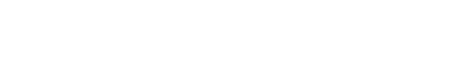
\includegraphics[width=0.29\textwidth]{figures/logos/logo-grs-dummy.png}%
    \hfill%
    
\includegraphics[width=0.1\textwidth]{figures/logos/logo-tum.png}%
}
}

\setbeamertemplate{title page}
{
	\vbox{}
	\vfill
	\begin{flushleft}
		\begin{beamercolorbox}[sep=8pt,center]{title}
			\usebeamerfont{title}\inserttitle\par%
			\ifx\insertsubtitle\@empty%
			\else%
				\vskip0.25em%
				{\usebeamerfont{subtitle}\usebeamercolor[fg]{subtitle}\insertsubtitle\par}%
			\fi%
    	\end{beamercolorbox}%
    	\vskip1em\par
		\begin{beamercolorbox}[sep=8pt,center]{author}
		\usebeamerfont{author}\insertauthor
		\end{beamercolorbox}
		\begin{beamercolorbox}[sep=8pt,center]{institute}
		\usebeamerfont{institute}\insertinstitute
		\end{beamercolorbox}
		\begin{beamercolorbox}[sep=8pt,center]{date}
		\usebeamerfont{date}\insertdate
		\end{beamercolorbox}\vskip0.5em
		{\usebeamercolor[fg]{titlegraphic}\inserttitlegraphic\par}
	\end{flushleft}
	\vfill
}

\mode<presentation>

\title{Configuration of a linear solver for linearly
	implicit time integration and efficient data
	transfer in parallel thermo-hydraulic
	computations
}

\author{Ravil Dorozhinskii}
\institute[]{Computational Science and Engineering}

% conditionals
\newif\ifSpeech
\newif\ifPresentation
\newif\ifCommentInclude
\newif\ifWithResults

\Speechfalse
\Presentationtrue
\CommentIncludefalse
\WithResultsfalse

\beamertemplatenavigationsymbolsempty

\setbeamertemplate{headline}
{
  \leavevmode%
  \hbox{%
  \begin{beamercolorbox}[wd=.6\paperwidth,ht=2.25ex,dp=1ex,center]{author in head/foot}%
    \usebeamerfont{subsection in head/foot}\insertsectionhead
  \end{beamercolorbox}%

  \begin{beamercolorbox}[wd=.2\paperwidth,ht=2.25ex,dp=1ex,center]{author in head/foot}%
    \usebeamerfont{institute in head/foot} TUM Informatics: CSE
  \end{beamercolorbox}%
  
  \begin{beamercolorbox}[wd=.2\paperwidth,ht=2.25ex,dp=1ex,center]{author in head/foot}%
    \usebeamerfont{author in head/foot}\insertframenumber{} / \inserttotalframenumber\hspace*{2ex}
  \end{beamercolorbox}
  }%
  \vskip0pt%
}

\makeatletter



\AtBeginSection[]{
  \begin{frame}
  \vfill
  \centering
  \begin{beamercolorbox}[sep=8pt,center,shadow=true,rounded=true]{title}
    \usebeamerfont{title}\insertsectionhead\par%
  \end{beamercolorbox}
  \vfill
  \end{frame}
}

\ifCommentInclude
\AtBeginSubsection[]{
  \begin{frame}
  \vfill
  \centering
  \begin{beamercolorbox}[sep=8pt,center,shadow=true,rounded=true]{title}
    \usebeamerfont{title}\insertsubsectionhead\par%
  \end{beamercolorbox}
  \vfill
  \end{frame}
}
\fi



\newcommand{\eq}[1]{Eq. \ref{#1}}
\newcommand{\fig}[1]{Fig. \ref{#1}}

\usepackage{bbding}
\newcommand{\extendadd}{\mbox{\: \CrossClowerTips \:}}


\begin{document}

%%%%%%%%%%%%%%%%%%%% INTRO %%%%%%%%%%%%%%%%%%%%
\begin{frame}
    \titlepage
\end{frame}


%\begin{frame}[t]
\frametitle{1-1: Title}

\begin{itemize}
    \item GRS has been the main German scientific research institute 
    
    \begin{itemize}
        \item in radioactive waste management
        \item and nuclear safety
        \item sine 1977
    \end{itemize}
    

    \item The organization develops and provides 
    \begin{itemize}
        \item \textbf{software products} for 
        \item \textbf{numerical simulation} of physical processes inside different \textbf{facilities of nuclear power plants}.\\
    \end{itemize}
\end{itemize}

\end{frame}


%%%%%%%%%%%%%%%%%%%%%%%%%%%%%%%%%%%%%%%%%%%%%%%%%%%%%%%%%%%%
\begin{frame}[t]
\frametitle{1-2: Title}
\justifying


\begin{itemize}
    \item ATHLE
    \item ATHLET\-CD 
    \item ATLAS
    \item COCOSYS
    \item DORT/TORT 
    \item QUABOX/CUBBOX

    \setlength\itemsep{0.5cm}
    \item The \textbf{main focus} of this study is dedicated to \textbf{ATHLET} software package as well as its \textbf{Numerical Toolkit}. 
    
    \item The \textbf{goal} of the study is to 
        \begin{itemize}
        \setlength\itemsep{0.5cm}
            \item \textbf{identify} the most \textbf{compute-intensive parts} of the ATHLET-NuT code 
            
            \item possibly \textbf{accelerate its execution time}\\
        \end{itemize}
\end{itemize}
\end{frame}


\begin{frame}{Outline I}
    \small 
    \tableofcontents[sections={1-4}]
\end{frame}

%%%%%%%%%%%%%%%%%%%% SOFTWARE %%%%%%%%%%%%%%%%%%%%
\section{Overview of ATHLET and NuT software}


\subsection{ATHLET}
\ifSpeech
%%%%%%%%%%%%%%%%%%%%%%%%%%%%%%%%%%%%%%%%%%%%%%%%%%%%%%%%%%
\begin{frame}[t]{3: Overview of ATHLET and NuT software}
  \justifying
  
  \begin{itemize}
    \setlength\itemsep{0.5cm}
      \item ATHLET is a thermal-hydraulic system simulation code
      
      \item developed for the analysis of the \textbf{whole spectrum} of \textbf{operational conditions}
      
      \item for nuclear energy facilities
      
    \item The code provides specific models and methods for the \textbf{simulation of many types of nuclear power plants} 
        \begin{itemize}
             \setlength\itemsep{0.5cm}
            \item including \textbf{current Light Water Reactors}
            \item and \textbf{advance 3rd and 4th generations}
        \end{itemize}
    
  \end{itemize}

\end{frame}

%%%%%%%%%%%%%%%%%%%%%%%%%%%%%%%%%%%%%%%%%%%%%%%%%%%%%%%%%%
\begin{frame}[t]{4: Mathematical Model: before equations}
    \justifying
    
    \begin{itemize}
        \setlength\itemsep{0.5cm}
    
        \item \textbf{Physical processes} inside of \textbf{hydraulic circuits} of light-water reactors
        
        \item can be naturally described by a \textbf{two-phase thermo-fluiddynamic model}
        
        \item  based on conservation equations of mass, momentum and energy for liquid and vapor.
    \end{itemize}

\end{frame}
\fi


%%%%%%%%%%%%%%%%%%%%%%%%%%%%%%%%%%%%%%%%%%%%%%%%%%%%%%%%%%
\ifPresentation
\begin{frame}[t]{Mathematical Model}
    \spc
    \justifying
    \small
    
1. Liquid mass
\begin{equation} \label{eq:athlet-1}
\frac{\partial ((1-\alpha)\rho_{l})}{\partial t} + \nabla ((1-\alpha) \rho_{l} \vec{w_{l}}) = - \psi
\end{equation}


2. Vapor mass
\begin{equation} \label{eq:athlet-2}
\frac{\partial (\alpha \rho_{v})}{\partial t} + \nabla (\alpha \rho_{v} \vec{w_{v}}) = \psi
\end{equation}


3. Liquid momentum
\begin{equation} \label{eq:athlet-3}
\frac{\partial ((1-\alpha) \rho_{l} \vec{w_{l}})}{\partial t} + \nabla ((1-\alpha) \rho_{l} \vec{w_{l}} \vec{w_{l}}) + \nabla ((1 - \alpha)p) = \vec{F_{l}}
\end{equation}

4. Vapor momentum
\begin{equation} \label{eq:athlet-4}
\frac{\partial (\alpha \rho_{v} \vec{w_{v}})}{\partial t} + \nabla (\alpha \rho_{v} \vec{w_{v}} \vec{w_{v}}) + \nabla (\alpha p) = \vec{F_{v}}
\end{equation}

    \normalsize
\end{frame}


\begin{frame}[t]{Mathematical Model}
    \spc
    \justifying
    \small
5. Liquid energy
\begin{equation} \label{eq:athlet-5}
\frac{\partial \Big[ (1-\alpha)\rho_{l}(h_{l} + \frac{1}{2} \vec{w_{l}} \vec{w_{l}} - \frac{p}{\rho_{l}}) \Big]}{\partial t} + \nabla \Big[ (1-\alpha)\rho_{l}\vec{w_{l}}(h_{l} + \frac{1}{2} \vec{w_{l}} \vec{w_{l}}) \Big] = - p \frac{\partial (1 - \alpha)}{\partial t} + E_{l}
\end{equation}


6. Vapor energy
\begin{equation} \label{eq:athlet-6}
\frac{\partial \Big[ \alpha \rho_{v}(h_{v} + \frac{1}{2} \vec{w_{v}} \vec{w_{v}} - \frac{p}{\rho_{v}}) \Big]}{\partial t} + \nabla \Big[ \alpha\rho_{v}\vec{w_{v}}(h_{v} + \frac{1}{2} \vec{w_{v}} \vec{w_{v}}) \Big] = - p \frac{\partial \alpha}{\partial t} + E_{v}
\end{equation}

7. Volume vapor fraction
\begin{equation} \label{eq:athlet-7}
	\alpha = \frac{V_{v}}{V}
\end{equation}

    \normalsize
    \spc
    \textit{According to \cite{lt:ATHLMaM}}\\
\end{frame}


%%%%%%%%%%%%%%%%%%%%%%%%%%%%%%%%%%%%%%%%%%%%%%%%%%%%%%%%%%
\begin{frame}[t]{Mathematical Model: from PDEs to ODEs}

    \begin{columns}
        \column{0.47\textwidth}
            \begin{figure}[htpb]
                \centering
                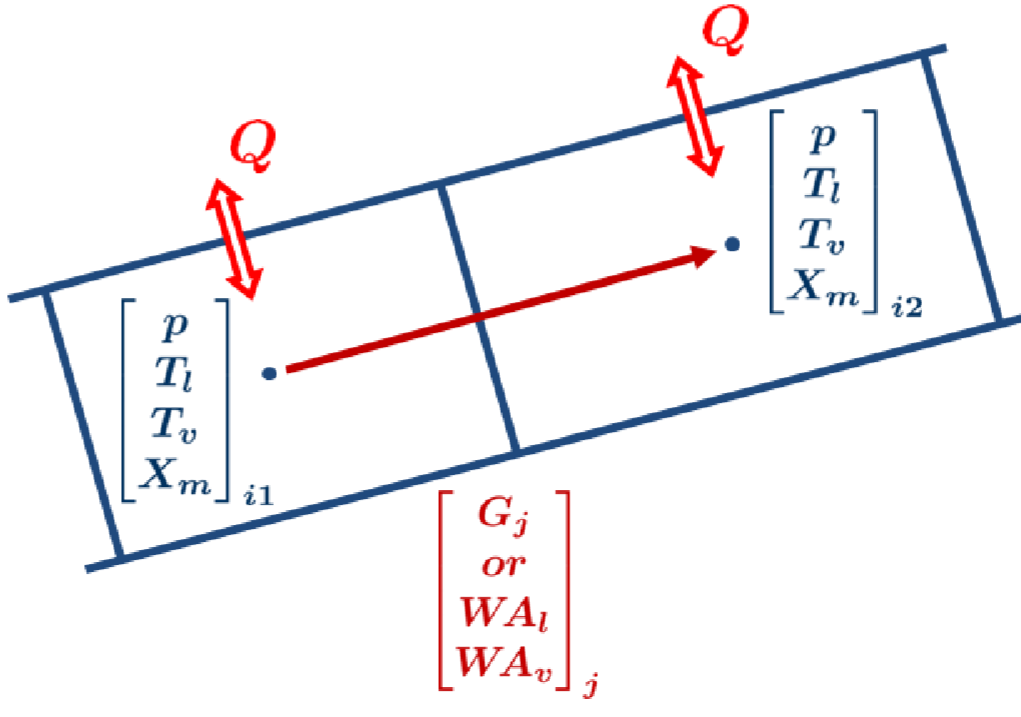
\includegraphics[width=0.8\textwidth]{figures/introduction-1d-fvm.png}
                \caption{ATHLET: one dimensional \textbf{Finite Volume} formulation of the problem \cite{tims-presentation}}
                \label{fig:introduction-1d-fvm}
            \end{figure}
        
        
        \column{0.5\textwidth}
        \justifying
        The system is transformed to a non-autonomous system of \textbf{ordinary differential equations} and expressed as an \textbf{initial value problem} after spatial finite-volume integration and some mathematical transformations \cite{lt:ATHLMaM}.
        
        
        \small
        \begin{equation} \label{eq:athlet-8}
	        \frac{dy}{dt} = f(t,y), \;  t_{0} \leq t \leq t_{F} \; y(t_{0}) = y_{0}
        \end{equation}
        \normalsize

        where $y \in \mathbb{R}^{N}$ is a composite vector of variables, $f$ is a non-linear function such that $f : \mathbb{R} \times \mathbb{R}^{N} \supset \Omega  \rightarrow \mathbb{R}^{N}$  .\\

    \end{columns}

\end{frame}

\fi

\ifSpeech
%%%%%%%%%%%%%%%%%%%%%%%%%%%%%%%%%%%%%%%%%%%%%%%%%%%%%%%%%%
\begin{frame}[t]{6: Mathematical Model: after equations}
    \justifying
    
    \begin{itemize}
        \setlength\itemsep{0.5cm}
    
        \item The system is \textbf{transformed} to a \textbf{non-autonomous} system of ODEs
        
        \item \textbf{expressed} as an \textbf{initial value problem}
        
        \item  After 
        
        \begin{itemize}
            \item Spatial Finite-Volume Integration
            
            \item some \textbf{advanced mathematical transformations}
        \end{itemize}
        
    \end{itemize}

\end{frame}

%%%%%%%%%%%%%%%%%%%%%%%%%%%%%%%%%%%%%%%%%%%%%%%%%%%%%%%%%%
\begin{frame}[t]{7-1: Numerical Integration: 6-stage W-method
}
    \justifying

    \begin{itemize}
        \setlength\itemsep{0.5cm}
        
        \item Analysis of the system shows the problem is stiff 
        
        \item hence, must to be solved with an implicit solver
        
        \item ATHLET uses a \textbf{6-stage W-method}
        
        \item which \textbf{belongs} to the \textbf{family of Linearly Implicit Method} 
        
        \item in particular \textbf{Rosenbrock methods}
        
        \item the method can be viewed as following
    \end{itemize}
    
\end{frame}



\begin{frame}[t]{7-2: Numerical Integration: 6-stage W-method}

    \justifying
  

        \begin{itemize}
            \setlength\itemsep{0.5cm}
            \item \textbf{Number} of stages determines the \textbf{oder} of the method
            \item Each stage is solved via \textbf{Implicit Euler method}
            \item Only \textbf{one Newton's} iteration is used for Imolicit Euler step 
            \item In contrast to the Rosenbrock methods, W-methods uses a \textbf{Jacobian matrix approximation}
        \end{itemize}

    \normalsize
\end{frame}

\fi


%%%%%%%%%%%%%%%%%%%%%%%%%%%%%%%%%%%%%%%%%%%%%%%%%%%%%%%%%%
\ifPresentation
\begin{frame}[t]{Numerical Integration: 6-stage W-method}
    \justifying
    
    \begin{equation}
        (I - h_{i}J)\delta y_{ij} = h_{i} f(t_{0} + j \cdot h_{i}, y_{0} + \sum^{j-1}_{l = 0} \delta y_{il}) + h^{2} \frac{\partial f_{0}}{\partial t}
    \end{equation}
    
    where $j=0, \dots, i - 1$; $h_{i} = h / i$; $i = 1, 2, 3$

    \begin{figure}[htpb]
          \centering
          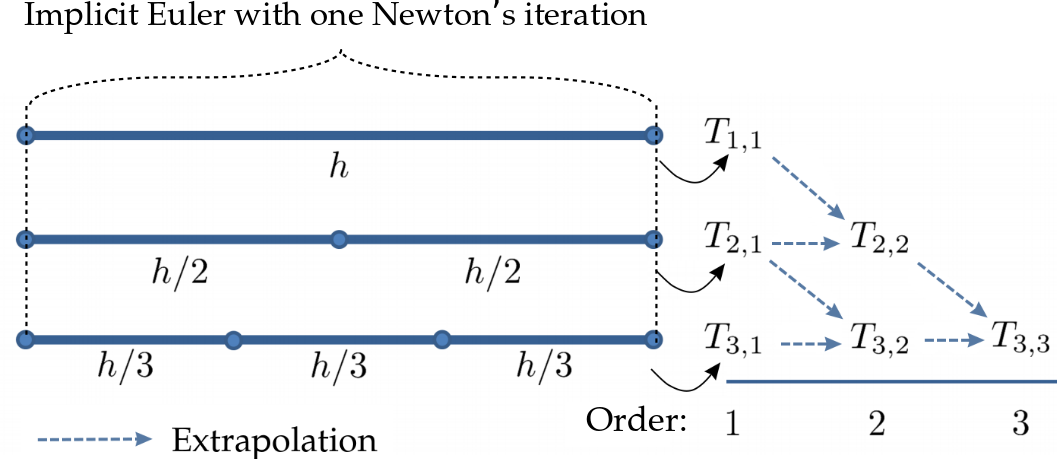
\includegraphics[width=0.8\textwidth]{figures/introduction-rosenbrock-scheme.png}
        \caption{A general view on 6-stage W-method \cite{tims-presentation}}
        \label{fig:introduction-w-method-scheme}
    \end{figure}

\end{frame}

\fi

\subsection{NuT}

%%%%%%%%%%%%%%%%%%%%%%%%%%%%%%%%%%%%%%%%%%%%%%%%%%%%%%%%%%
\ifSpeech
\begin{frame}[t]{8-1: NuT Purpose and Architecture}
    \spc
    \justifying
    
    \begin{itemize}
        \setlength\itemsep{0.25cm}
        \item Numerical Toolkit is a \textbf{container} of various \textbf{dense and sparse} linear algebra \textbf{subroutines}
        
        \item the main focus is \textbf{parallel execution} on distributed-memory machine
        
        \item based on Portable, Extensible Toolkit for Scientific Computation \textbf{PETSc}
        
        \item NuT design follows the paradigm of \textbf{Adapter/Wrapper} pattern which provides \textbf{uniform common interface} for its services 
        
        \item to achieve \textbf{re-usability}, flexibility and extensibility properties of the code
    \end{itemize}

\end{frame}
\fi



%%%%%%%%%%%%%%%%%%%%%%%%%%%%%%%%%%%%%%%%%%%%%%%%%%%%%%%%%%
\ifSpeech
\begin{frame}[t]{8-2: NuT Purpose and Architecture}
    \justifying
    
        Example ATHLET-NuT:
         \begin{itemize}
            \setlength\itemsep{0.25cm}
         
            \item ATHLET is responsible for \textbf{marching} of the numerical \textbf{integration solver}
            
            \item ATHLET computes a \textbf{Jacobian} matrix approximation and the \textbf{right-hand sides}
            
            \item NuT  \textbf{solves systems} of linear equation
        \end{itemize}

        
        \vspace{0.75cm}
        Communication or Software Coupling:
        \begin{itemize}
            \setlength\itemsep{0.25cm}
            \item Implemented by means of \textbf{MPI}
            
            \item Communication is \textbf{synchronous} 
        \end{itemize}

        

\end{frame}



%%%%%%%%%%%%%%%%%%%%%%%%%%%%%%%%%%%%%%%%%%%%%%%%%%%%%%%%%%
\begin{frame}[t]{9: NuT Multi-client mode}
    \justifying
    
    \begin{itemize}
    
        \setlength\itemsep{0.5cm}
        \item \textbf{Client-server} architecture is used 
        
        \item to \textbf{provide software coupling} between NuT and other GRS tools

        \item  The design allows \textbf{sharing} of some NuT-MPI processes \textbf{among} different \textbf{process groups}
        
        \item usually happens due to the finite number of processors on hardware e.g. laptops, PC, etc.
        
        \item it is better to avoid sharing 
    \end{itemize}
    
    
\end{frame}
\fi




\section{Problem Statement}

%%%%%%%%%%%%%%%%%%%%%%%%%%%%%%%%%%%%%%%%%%%%%%%%%%%%%%%%%%
\ifPresentation
\begin{frame}[t]{Solving Sparse Linear Systems}
    \small
    \justifying
    Numerical \textbf{integration} of a system of ODEs by means of \textbf{W-methods}:
    
    \begin{equation}
	(I - h_{i}J)\delta y_{ij} = h_{i} f(t_{0} + j \cdot h_{i}, y_{0} + \sum^{j-1}_{l = 0} \delta y_{il}) + h^{2} \frac{\partial f_{0}}{\partial t}
    \end{equation}
    
    can be considered as a solution of a \textbf{sequence of linear systems} from another point of view:
    
    \begin{equation}
	A_{i} \delta y_{ij} =  b_{ij} 
    \end{equation}

    where $A = (I - h_{i}J)$ is a $\mathbb{R}^{N} \times \mathbb{R}^{N}$ non-singular \textbf{sparse matrix}; $\delta y_{ij}$  and $b_{ij}$ are $\mathbb{R}^{N}$ vectors; $i = 1, 2, 3$; $j=0, \dots, i - 1$\\
    
    \begin{block}{NOTE}
        Computational \textbf{burden} of the W-method mainly lies in \textbf{solving of sparse linear systems} beside evaluation of non-linear function $f$ of \eq{eq:athlet-8}
    \end{block}

\end{frame}
\fi

\ifSpeech
%%%%%%%%%%%%%%%%%%%%%%%%%%%%%%%%%%%%%%%%%%%%%%%%%%%%%%%%%%
\begin{frame}[t]{11: Solving Sparse Linear Systems}

    \justifying

    \textbf{Efficient} numerical integration governed by W-methods \textbf{demenads} the following \textbf{properties} of a linear sparse solver:
    
    \begin{itemize}
	    \item robustness (or numerical stability) with respect to ill-conditioner problems
    	\item parallel efficiency, with emphasis on strong scaling 
    \end{itemize}
    \spc
    
    
    \textbf{Extra constrains} imposed by the project:
    
    \begin{itemize}
    	\item open-source license
    	\item direct interface to PETSc
    \end{itemize}
    
    \begin{block} {MENTION}
        \textbf{These Can be considered as Non-Functional requirements}    
    \end{block}
    
    
\end{frame}
\fi






%%%%%%%%%%%%%%%%%%%%%%%%%%%%%%%%%%%%%%%%%%%%%%%%%%%%%%%%%%
\ifSpeech
\begin{frame}{Problem Statement}
    \spc
    \justifying
    
    \begin{block}{Goals of the study}
        \begin{enumerate}
            \setlength\itemsep{0.5cm}
            \item Find and configure a parallel sparse linear solver
            
            \item Improve ATHLET-NuT communication during Jacobian matrix transfers
        \end{enumerate}
    \end{block}

\end{frame}
\fi
\section{Methodology and Matrix Sets}


%%%%%%%%%%%%%%%%%%%%%%%%%%%%%%%%%%%%%%%%%%%%%%%%%%%%%%%%%%
\begin{frame}[t]{Static Solver Configuration}
    \footnotesize
    \justifying
    \begin{itemize}
        \setlength\itemsep{0.25cm}
        \item ATHLET is a CFD tool dedicated to \textbf{transient problems}
        \item Additionally, \textbf{topology} of hydrolic circuits can \textbf{be changed} during simulation-time
        \item Hence, the Jacobian matrix \textbf{structure} can \textbf{vary} significantly during numerical itegration
    \end{itemize}
    
    \small
    \begin{block}{Therefore:}
        \begin{enumerate}
            \item Configuration of a linear solver in run-time is compute-intensive and time consuming
            
            \item Reults of dynamic solver configuration can be ambiguous and difficult to interpret
            
            \item A feasible and doable approach is \textbf{static solver configuration}
        \end{enumerate}
    \end{block}

\end{frame}

%%%%%%%%%%%%%%%%%%%%%%%%%%%%%%%%%%%%%%%%%%%%%%%%%%%%%%%%%%
\begin{frame}[t]{GRS Matrix Set}
    \spc
    \justifying
    
    GRS \textbf{matrix set} was generated by \textbf{running} the most \textbf{common GRS simulations} in ATHLET and \textbf{stopping} them \textbf{somewhere in the middle}. The corresponding shifted Jacobian matrices ware saved in the PETSc binary format.
    
    \begin{table}[ht]
        \small
        \centering
        \begin{tabular}{|c|c|c|c|c|}
        \hline
        Name     & n       & nnz      & nnz / n & \begin{tabular}[c]{@{}c@{}}Approximate\\ Condition\\ Number\end{tabular} \\ \hline
        pwr-3d   & 6009    & 32537    & 5.4147  & 1.019e+07
         \\ \hline
        cube-5   & 9325    & 117897   & 12.6431 & 1.592e+09                                                                \\ \hline
        cube-64  & 100657  & 1388993  & 13.7993 & 7.406e+08                                                                \\ \hline
        cube-645 & 1000045 & 13906057 & 13.9054 & 6.474e+08
         \\ \hline
        k3-2     & 130101  & 787997   & 6.0568  & 1.965e+15                                                                \\ \hline
        k3-18    & 1155955 & 7204723  & 6.2327  & 1.947e+12                                                                \\ \hline
        \end{tabular}
        \caption{GRS matrix set}
        \label{table:grs-matrix-set}
\end{table}

\end{frame}


%%%%%%%%%%%%%%%%%%%%%%%%%%%%%%%%%%%%%%%%%%%%%%%%%%%%%%%%%%
\begin{frame}[t]{SuiteSparse Matrix Set}
    \spc
    \justifying
    \textbf{SiteSparse} matrix set was generated by \textbf{downloading} a dozen of matrices from SuiteSparse Matrix Collection \cite{sparse-matrix-collection:1}, \cite{sparse-matrix-collection:2}, with the \textbf{aim} of \textbf{comparison} and \textbf{verification} of solver configurations
    
    \begin{table}[ht]
\centering
\footnotesize
\begin{tabular}{|c|c|c|c|c|c|}
\hline
Name        & n       & nnz      & nnz / n & \begin{tabular}[c]{@{}c@{}}Approximate\\ Condition\\ Number\end{tabular} \\ \hline
cant        & 62451   & 4007383  & 64.1684 & 5.082e+05\\ \hline
consph      & 83334   & 6010480  & 72.1251 & 2.438e+05\\ \hline
CurlCurl\_3 & 1219574 & 13544618 & 11.1060 & 2.105e+05\\ \hline
Geo\_1438   & 1437960 & 63156690 & 43.9210 & 4.677e+05\\ \hline
memchip     & 2707524 & 13343948 & 4.9285  & 1.305e+07\\ \hline
PFlow\_742  & 742793  & 37138461 & 49.9984 & 5.553e+06\\ \hline
pkustk10    & 80676   & 4308984  & 53.4110 & 5.589e+02\\ \hline
torso3      & 259156  & 4429042  & 7.0903  & 2.456e+03\\ \hline
x104        & 108384  & 8713602  & 80.3956 & 3.124e+05\\ \hline
\end{tabular}
\caption{SuiteSparse matrix set}
\label{table:suite-sparse-matrix-set}
\end{table}

\end{frame}


%%%%%%%%%%%%%%%%%%%%%%%%%%%%%%%%%%%%%%%%%%%%%%%%%%%%%%%%%%

\begin{frame}[t]{Hardware}
    \begin{table}[ht]
\centering
\footnotesize
\begin{tabular}{|l|c|c|}
\hline
                    & HW1 (GRS) & HW2 (LRZ Linux) \\ \hline
CPU(s)              & 20 &  28 \\ \hline
On-line CPU(s) list & 0-19 &  0-27 \\ \hline
Thread(s) per core  & 1 &  1 \\  \hline
Core(s) per socket  & 10 & 14 \\ \hline
Socket(s)           & 2 &  2 \\ \hline
NUMA node(s)        & 2 &  4 \\ \hline
Model name          & E5-2680 v2 & 
E5-2697 v3 \\ \hline
Stepping            & 4 &  2 \\ \hline
CPU MHz             & 1200.0 &  2036.707 \\ \hline
L1 d/i cache        & 32K/32K &  32K/32K \\ \hline
L2 cache            & 256K &  256K \\ \hline
L3 cache            & 25600K &  17920K \\ \hline
NUMA node0 CPU(s)   & 0-9 &  0-6 \\ \hline
NUMA node1 CPU(s)   & 10-19 &  7-13 \\ \hline
NUMA node2 CPU(s)   & - &  14-20 \\ \hline
NUMA node3 CPU(s)   & - &  21-27 \\ \hline
\end{tabular}
\caption{Hardware specification}
\label{table:hardware-spec}
\end{table}
    
\end{frame}





%%%%%%%%%%%%%%%%%%%%%%%%%%%%%%%%%%%%%%%%%%%%%%%%%%%%%%%%%%
\begin{frame}{Experimental setup}

    \justifying
    
    \begin{block} {Libraries and Compiler}
        \begin{enumerate}
            \item PETSc version 3.10
        \item OpenMPI version 3.1.1
            \item Intel Compiler 18
        \end{enumerate}
    \end{block}

\end{frame}



%%%%%%%%%%%%%%%%%%%% TASK 1 %%%%%%%%%%%%%%%%%%%%


%\AtBeginSubsection[]{}
\AtBeginSection[]{}

\section{Overview of Sparce linear Solver Types}
  \subsection{Iterative Methods}
    \subsubsection{Theory overview}
    \subsubsection{Parallelization Aspects}
    \subsubsection{Preconditioners}
  
  \subsection{Direct Sparse Methods}
    \subsubsection{Theory overview}
    \subsubsection{Parallelization Aspects}
    \subsubsection{Theshold Pivoting and Solution Refinement}

  \subsection{Conclusion}
  
\section{Selection Of Sparse Direct Solver Library}
\section{Configuration of MUMPS library}
  \subsection{Overview of MUMPS}
  \subsection{Fill reducing Reorderings}
  \subsection{MPI Process pinning}
  \subsection{Optimized of BLAS library}
  \subsection{Hybrid MPI-OpenMP computing}
  \subsection{Conclusion}

%%%%%%%%%%%%%%%%% THEORY %%%%%%%%%%%%%%

\section{Overview of Solver Types}
% Iterative methods
\subsection{Iterative Methods}
\subsubsection{Theory overview}

%%%%%%%%%%%%%%%%%%%%%%%%%%%%%%%%%%%%%%%%%%%%%%%%%%%%%%%%%%
\begin{frame}[t]{Iterative methods}
    \small
    
    \begin{itemize}
    	\item Given an initial guess
    	
    	\item An iterative method generates a sequence of approximate solutions by means of a specific rule
    	
    	\item Depending on a method and the given problem,
    	
    	\item there may exist certain conditions such that the sequence eventually converges to the exact solution
    	
    \end{itemize}

    \begin{itemize}
    	\item There exist two families of iterative methods: \textit{stationary} and \textit{Krylov-based} methods
    	
    	\item Nowadays, Krylov methods dominate in the field of scientific computing
    	
    	\begin{itemize}
    		\item because of their rather fast convergence
    		
    		\item in case of solving well conditioned systems
    		
    		\item or/and a "\textit{good}" initial guess
    	\end{itemize}
    \end{itemize}

\end{frame}


\begin{frame}[t]{Krylov-based methods}
    \small
    \begin{itemize}
    	\item \textit{The key idea} is to construct an approximate solution 
    	\item as a linear combination of vectors $b$, $Ab, \:\: A^2b, \:\: A^3b, \dots A^{n-1}b$
    	\item known as Krylov subspace $\mathcal{K}_{n}$
    	
    	\item where, without of lost of generality, the initial guess $x_0$ is equal to zero
    	
    	\item At each iteration, the subspace is expanded by adding and evaluating the next vector in the sequence
    \end{itemize}

	\begin{itemize}
		\item the methods define and expand another subspace $\mathcal{L}_{n}$ 
		
		\item such that $r_{n} = b - Ax_{n} \perp \mathcal{L}_{n}$ 
		
		\item which is known as the Petrov-Galerkin condition
		
		\item A construction of subspace $\mathcal{L}_{n}$ is defined by a method
		
		\item and based on matrix properties
		
	\end{itemize}
\end{frame}
\subsubsection{Aspects}

%%%%%%%%%%%%%%%%%%%%%%%%%%%%%%%%%%%%%%%%%%%%%%%%%%%%%%%%%%
\ifSpeech
\begin{frame}[t]{Parallelization Aspects: Speech}
    \small
    \justifying
    \begin{itemize}
    	\item Iterative methods usually make use of simple linear algebra kernels e.g. dot products, matrix-vector products, etc.
    	
    	\begin{itemize}
    		\item Therefore, sparsity of linear systems can be handled well
    	\end{itemize}
    	
    	\item The methods make use of data-based parallelism
    	
    	\begin{itemize}
    		\item vectors and matrices are distributed among multiple processing units
    		
    		\item Therefore, the methods scales well in parallel
    		
    		\item the main drop of parallel performance mainly
comes from process-communication overheads	
    	\end{itemize}
    	
    \end{itemize}   
\end{frame}

\begin{frame}[t]{Preconditioners: Speech}
\small
\justifying

\begin{itemize}
	\item In case of a "bad" initial guess $x_{0}$, convergence of iterative methods strongly depends on an involved matrix and, in particular, on its condition number
	
	\item A big condition number usually leads to slow convergence
	
	\item a linear transformation, known as preconditioning, can be applied to the original system of equations
	
	\item to reduce its condition number and, therefore, to accelerate convergence
\end{itemize}

\begin{itemize}
	\item a good preconditioning algorithm should result in
	
	\begin{itemize}
		\item low computational cost
		\item low storage space 
		\item low condition number of the transformed system
		\item adapted for parallel executions as well
	\end{itemize}
\end{itemize}
\end{frame}
\fi


\begin{frame}[t]{Aspects}
\small
\begin{block}{Parallelization Aspects}
	
	\begin{itemize}
		\item Iterative methods usually make use of simple linear algebra kernels e.g. dot products, matrix-vector products, etc.
		
		\item Therefore, the methods efficiently make use of data-based parallelism 
	\end{itemize}
\end{block}

\begin{block}{Numerical Accuracy}
	
	\begin{itemize}
		\item Convergence to the exact solution depends on a value of the  condition number of a matrix
		
		\item Usually requires a linear transformation known as preconditioning
		
		\begin{itemize}
			\item to reduce condition number and accelerate convergence
		\end{itemize}
	\end{itemize}
\end{block}
\end{frame}


\begin{frame}[t]{Preconditioners}
\tiny
\begin{table}[!t]
	\tiny
	\centering
	\begin{tabular}{|c|c|c|c|c|}
		\hline
		\begin{tabular}[c]{@{}c@{}}Package\\ name\end{tabular}     & Origin                                                   & Method                                                        & \begin{tabular}[c]{@{}c@{}}Tuning\\ parameters\end{tabular}                                                                                                                            & Comments                                                                  \\ \hline
		block Jacobi                                               & PETSc                                                    & block Jacobi                                                  & \begin{tabular}[c]{@{}c@{}}-pc\_bjacobi\_blocks\\ -sub\_pc\_type\end{tabular}                                                                                                          & -                                                                         \\ \hline
		\begin{tabular}[c]{@{}c@{}}additive\\ Schwarz\end{tabular} & PETSc                                                    & \begin{tabular}[c]{@{}c@{}}additive\\ Schwarz\end{tabular}    & \begin{tabular}[c]{@{}c@{}}-pc\_asm\_blocks\\ -pc\_asm\_overlap\\ -pc\_asm\_type\\ -pc\_asm\_local\_type\\ -sub\_pc\_type\end{tabular}                                                 & -                                                                         \\ \hline
		euclid                                                     & hypre                                                    & ILU(k)                                                        & \begin{tabular}[c]{@{}c@{}}-nlevel\\ -thresh\\ -filter\end{tabular}                                                                                                                    & \begin{tabular}[c]{@{}c@{}}deprecated\\ form\\ PETSc\end{tabular}         \\ \hline
		pilut                                                      & hypre                                                    & ILU(t)                                                        & \begin{tabular}[c]{@{}c@{}}-pc\_hypre\_pilut\_tol\\ -pc\_hypre\_pilut\_maxiter\\ -pc\_hypre\_pilut\_factorrowsize\end{tabular}                                                         & -                                                                         \\ \hline
		parasail                                                   & hypre                                                    & SPAI                                                          & \begin{tabular}[c]{@{}c@{}}-pc\_hypre\_parasails\_nlevels\\ -pc\_hypre\_parasails\_thresh\\ -pc\_hypre\_parasails\_filter\end{tabular}                                                 & -                                                                         \\ \hline
		SPAI                                                       & \begin{tabular}[c]{@{}c@{}}Grote,\\ Barnard\end{tabular} & SPAI                                                          & \begin{tabular}[c]{@{}c@{}}-pc\_spai\_epsilon\\ -pc\_spai\_nbstep\\ -pc\_spai\_max\\ -pc\_spai\_max\_new\\ -pc\_spai\_block\_size\\ -pc\_spai\_cache\_size\end{tabular}                & -                                                                         \\ \hline
		BoomerAMG                                                  & hypre                                                    & \begin{tabular}[c]{@{}c@{}}algebraic\\ multigrid\end{tabular} & \begin{tabular}[c]{@{}c@{}}-pc\_hypre\_boomeramg\_cycle\_type\\ -pc\_hypre\_boomeramg\_max\_levels\\ -pc\_hypre\_boomeramg\_max\_iter\\ -pc\_hypre\_boomeramg\_tol\\ etc.\end{tabular} & \begin{tabular}[c]{@{}c@{}}39 tuning\\ parameters\\ in total\end{tabular} \\ \hline
	\end{tabular}
	\caption{Parallel preconditioning algorithms available in PETSC}
	\label{table:preconditioners}
\end{table}

\end{frame}






%Direct methods
\subsection{Direct Sparse Methods}
\subsubsection{Theory overview}

%%%%%%%%%%%%%%%%%%%%%%%%%%%%%%%%%%%%%%%%%%%%%%%%%%%%%%%%%%
\begin{frame}[t]{Direct Sparse Methods}
    \small
    \justifying
    
    Direct sparse methods combine the main advantages of direct and iterative methods
    
    \begin{itemize}
    	\item numerical accuracy of the methods is comparable with the standard Gaussian Elimination process
    	
    	\item complexity is bounded by $O(n^{2})$ due to efficient treatment of sparsity
    \end{itemize}

	\vspace{5mm}
	A solution of a system of equations is computed:
	\begin{itemize}
		\item by means of forward and backward substitutions
		 
		\item using $LU$ decomposition of the corresponding matrix.
	\end{itemize}
\end{frame}


\begin{frame}[t]{Direct Sparse Methods: Speech}
	\small
	\justifying
	\begin{itemize}
		\item The multifrontal method is probably the most representative example of direct sparse solvers
		 introduced by Duff and Reid
		 
		 \item The method is an improved version of the frontal method 
		 
		 \item which can compute independent fronts in parallel. 
		 
		 \item A front, also called a frontal matrix, can be considered as a small dense matrix 
		 
		 \item resulting from a column elimination of the original system. 
		 
		 \item There also exist left- and right-looking vatiants of the multifrontal method
		 
	\end{itemize}

	\vspace{5mm}
	Let's consider the multifrontal methods as an example\\
	\vspace{2.5mm}
	To keep the overview rather simple, we assume that matrix $A$ is \textbf{symmetric positive definite} and \textbf{sparse}
	
	
	
\end{frame}


\begin{frame}[t]{Multifrontal Method: I}
	\small
	\justifying
		\begin{equation} \label{eq:chol-1}
		A = LDL^T \qquad \text{with}\quad (D)_{ii} > 0
		\end{equation}
		
		Given a rule and a sparsity pattern, one can build an elimination tree
		\begin{equation} \label{eq:elimination-tree-1}
			p = min(i > j | l_{ij} \neq 0)
		\end{equation}
		
	
	\vspace{-5mm}
		
	\begin{columns}
		\begin{column}{0.5\textwidth}
			\begin{figure}[!htpb]
				\centering
				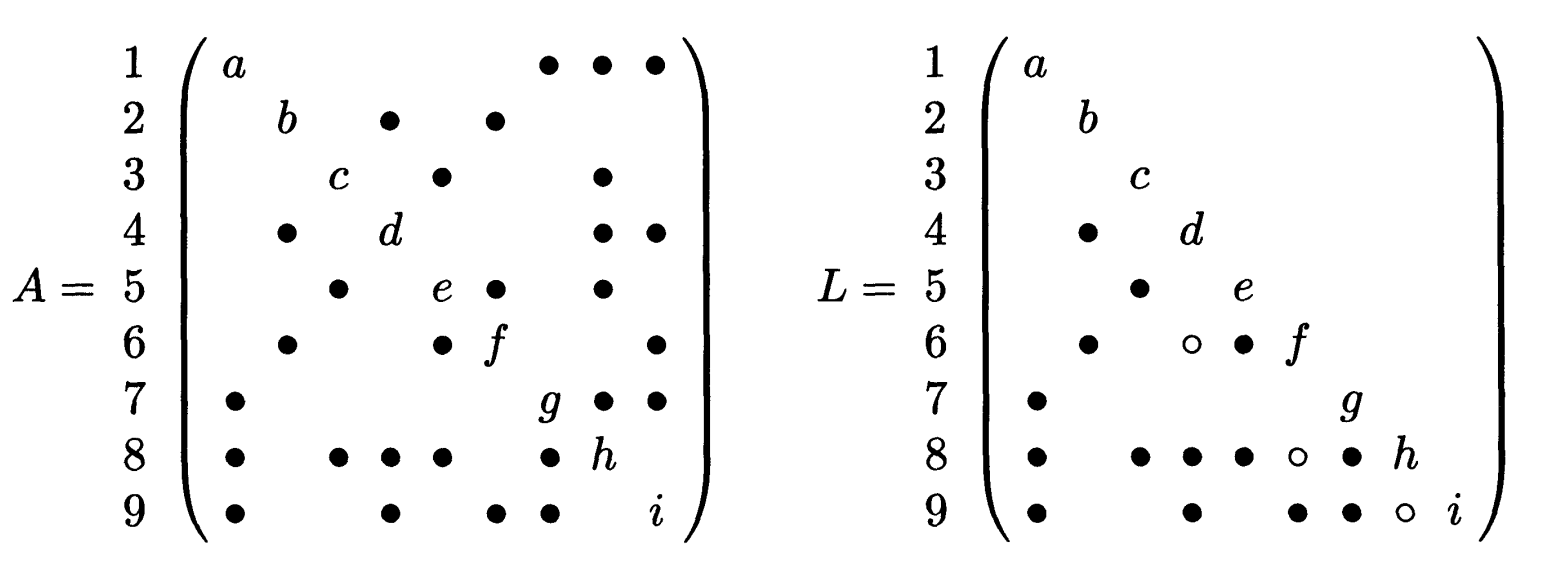
\includegraphics[width=1.2\textwidth]{figures/chapter-2/sparsity-pattern-example-mm.png}
				\caption{A sparse matrix and its Cholesky factor, \cite{mult-frontal-original:2}}
				\label{fig:sparsity-pattern-example-mm}
			\end{figure}
		\end{column}
			
		\begin{column}{0.5\textwidth}
			
			\begin{figure}[!htpb]
				\centering
				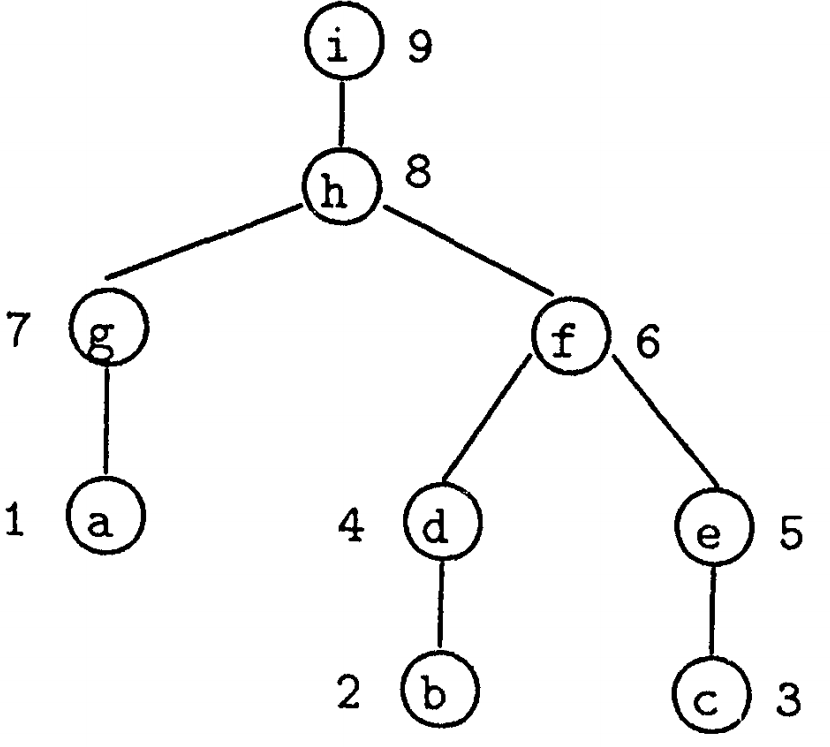
\includegraphics[width=0.65\textwidth]{figures/chapter-2/elimination-tree-mm.png}
				\caption{An elimination tree, \cite{mult-frontal-original:2}}
				\label{fig:elimination-tree-mm}
			\end{figure}
		\end{column}

	\end{columns}
	
	
\end{frame}


\begin{frame}[t]{Multifrontal Method: II}
	\small
	\justifying
	The fundamental idea of the multifrontal method spins around frontal $F$ and update matrices $\hat{U}$
	\begin{equation} \label{eq:mm-1}
		F_{j} = Fr_{j} + \hat{U_{j}} = \begin{bmatrix}a_{j,j} & a_{j,i_1} & a_{j,i_2} & \dots & a_{j,i_r} \\
		a_{i_1,j} \\
		a_{i_2,j} \\
		\vdots & & & 0\\
		a_{i_r,j} \\
		\end{bmatrix} + \hat{U_{j}}
	\end{equation}
	
	where $i_{0}$, $i_{1}$, $i_{2}$, \dots , $i_{r}$ are row subscripts of non-zeros in $L_{*j}$ where $i_{0} = j$; $r$ is the number of off-diagonal non-zero elements.\\


	\begin{equation} \label{eq:mm-2}
		\hat{U_{j}} = - \sum_{k \in T[j] -{j}}  \begin{bmatrix}
		l_{j,k} \\
		l_{i_1,k} \\
		\vdots \\
		l_{i_r,k} \\
		\end{bmatrix} \begin{bmatrix}
		l_{j,k} & l_{i_1,k} & \dots & l_{i_r,k}
		\end{bmatrix} 
	\end{equation}
	
	where $\hat{U_{j}}$ can be treated as the second term of the Schur complement
	
\end{frame}


\begin{frame}[t]{Multifrontal Method: III}
	\small
	\justifying
	Let's consider factorization of a 2-by-2 block matrix $A$
	\begin{equation} \label{eq:mm-3}
		A = \begin{bmatrix}
		B & V^{T} \\
		V & C
		\end{bmatrix} 
		= 
		\begin{bmatrix}
		L_{B} & 0 \\
		VL^{-T}_{B} & I
		\end{bmatrix}
		\begin{bmatrix}
		I & 0 \\
		0 & Sr
		\end{bmatrix} 
		\begin{bmatrix}
		L^{T}_{B} & L^{-1}_{B}V^{T} \\
		0 & I
		\end{bmatrix} 
	\end{equation}
	
	Assuming that block $B$ has already been factorized: $B = L_{B}L^{T}_{B}$\\
	
	\vspace{5mm}
	The Schur complement can be viewed as:
	\begin{equation} \label{eq:mm-3}
	Sr =  C - VB^{-1}V^{T}
	\end{equation}
	
	\begin{columns}
		\begin{column}{0.5\textwidth}
			\textit{Dense Linear Algebra:} $-VB^{-1}V^{T}$\\
			\begin{equation} \label{eq:mm-5}
				-\sum_{k=1}^{j-1}  \begin{bmatrix}
				l_{j,k} \\
				\vdots \\
				l_{n,k} \\
				\end{bmatrix} \begin{bmatrix}
				l_{j,k} & \dots & l_{n,k}
				\end{bmatrix} 
			\end{equation}
		\end{column}
	
		\begin{column}{0.5\textwidth}
			\textit{Multifrontal method:} $\hat{U_{j}}$\\
			\begin{equation} \label{eq:mm-2}
				-\sum_{k \in T[j] -{j}}  \begin{bmatrix}
				l_{i_0,k} \\
				\vdots \\
				l_{i_r,k} \\
				\end{bmatrix} \begin{bmatrix}
				l_{i_0,k} & \dots & l_{i_r,k}
				\end{bmatrix} 
			\end{equation}
		\end{column}
	\end{columns}
	
\end{frame}


\begin{frame}[t]{Multifrontal Method: IV}
	\small
	\justifying
	
	After column $j$ factorization:
	\begin{equation} \label{eq:mm-6}
		\hat{F_{j}} = \begin{bmatrix}
		l_{j,j} & \dots & 0 \\
		\vdots & I \\
		l_{i_{r},j} \\
		\end{bmatrix} 
		\begin{bmatrix}
		1 & \dots & 0 \\
		\vdots & U_{j} \\
		0 \\
		\end{bmatrix} 
		\begin{bmatrix}
		l_{j,j} & \dots & l_{i_{r},j} \\
		\vdots & I \\
		0 \\
		\end{bmatrix} 
	\end{equation}
	where sub-matrix $U_{j}$ represents the full update from all descendants of node $j$ and node $j$ itself
	
	
	\begin{columns}
		
	\begin{column}{0.25\textwidth}
		\begin{figure}[!htpb]
			\centering
			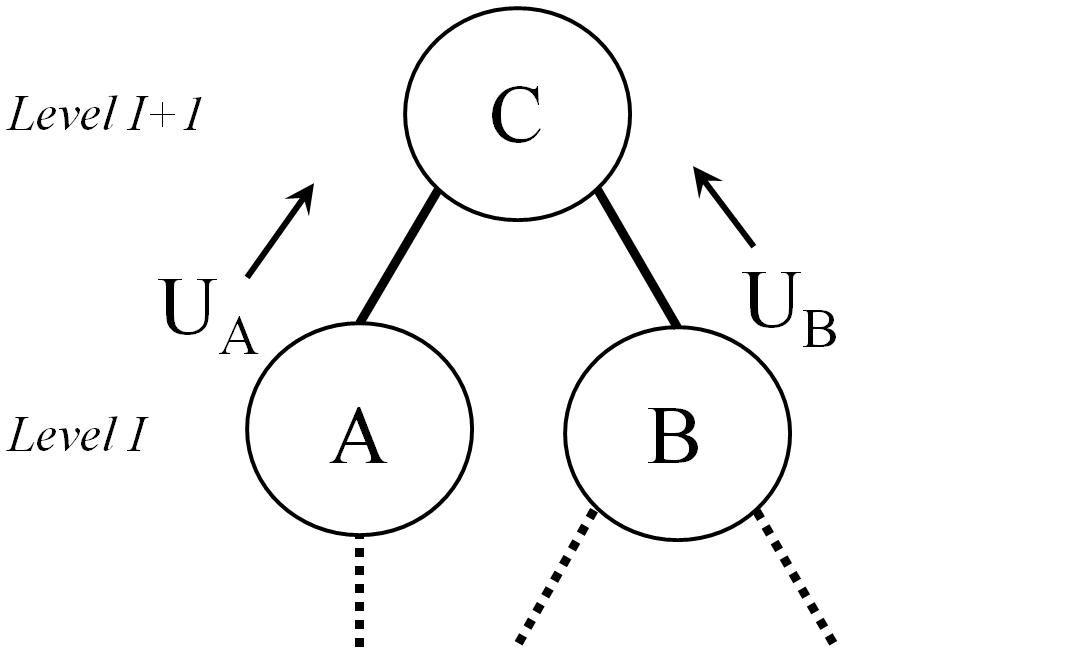
\includegraphics[width=1.35\textwidth]{figures/chapter-2/information-flow.png}
			\caption{Information flow}
			\label{fig:information-float}
		\end{figure}
	\end{column}

	\begin{column}{0.75\textwidth}
		\begin{equation} \label{eq:mm-9}
			F_{j} = \begin{bmatrix}a_{j,j} & a_{j,i_1} & a_{j,i_2} & \dots & a_{j,i_r} \\
			a_{i_1,j} \\
			a_{i_1,j} \\
			\vdots & & & 0\\
			a_{i_r,j} \\
			\end{bmatrix} \extendadd U_{c_1} \extendadd \dots \extendadd U_{c_s} 
		\end{equation}
	\end{column}

	\end{columns}
\end{frame}



\begin{frame}[t]{Supernodal Method}
	\small
	
	\begin{itemize}
		\item In practice, an improved version of the multifrontal method is used
		\item A super-node is formed by a set of contiguous columns 
		
		\item which have the same  off-diagonal sparsity structure
	\end{itemize}

	\begin{equation} \label{eq:mm-10}
		\mathcal{F}_{j} = \begin{bmatrix}a_{j,j} & a_{j,j+1} & \dots & a_{j,j+t}  & a_{j,i_1} & \dots & a_{j,i_r} \\
		a_{j+1,j} & a_{j+1,j+1} & \dots & a_{j+1,j+t}  & a_{j+1,i_1} & \dots & a_{j+1,i_r} \\
		\vdots & \vdots & \dots & \vdots \\
		a_{j+t,j}  & a_{j+t,j+1} & \dots & a_{j+t,j+t}  & a_{j+t,i_1} & \dots & a_{j+t,i_r} \\
		a_{i_1,j} & a_{i_1,j+1} & \dots & a_{i_1,j+t} \\
		\vdots & \vdots & \dots & \vdots  & & 0\\ 
		a_{i_r,j} & a_{i_r,j+1} & \dots & a_{i_r,j+t} \\
		\end{bmatrix} \extendadd U_{c_1} \dots \extendadd U_{c_s} 
	\end{equation}

\end{frame}
\subsubsection{Parallelization Aspects}

%%%%%%%%%%%%%%%%%%%%%%%%%%%%%%%%%%%%%%%%%%%%%%%%%%%%%%%%%%

\begin{frame}[t]{Parallelization Aspects}
\small

\vspace{-5mm}
\begin{columns}
	\begin{column}{0.5\textwidth}
		\begin{figure}
			\centering
			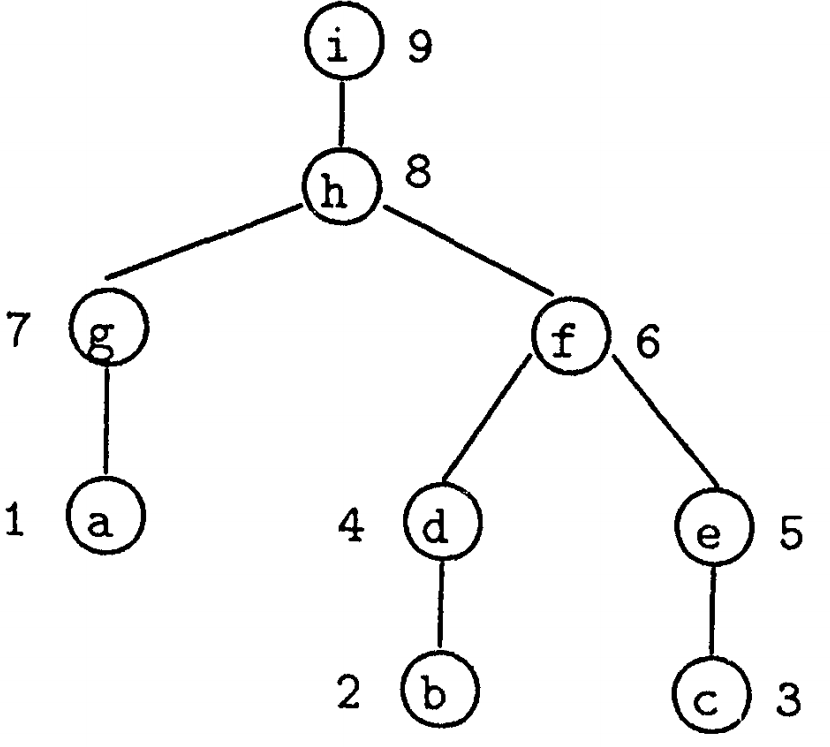
\includegraphics[width=0.3\textheight]{figures/chapter-2/elimination-tree-mm.png}
			\caption{Original elimination tree}
		\end{figure}
	\end{column}
	
	\begin{column}{0.5\textwidth}
		\begin{figure}
			\centering
			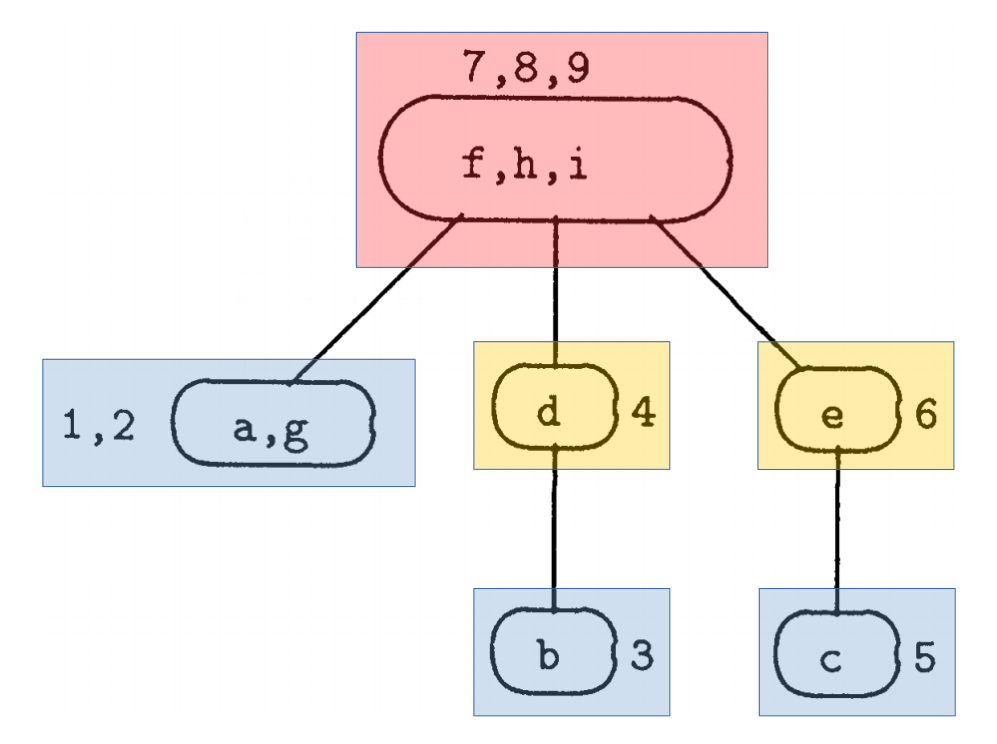
\includegraphics[width=0.6\textwidth]{figures/chapter-2/elimination-tree-parallel.png}
			\caption{Supernodal/assembly tree}
		\end{figure}
	\end{column}
	
\end{columns}

\begin{figure}[!htpb]
	\centering
	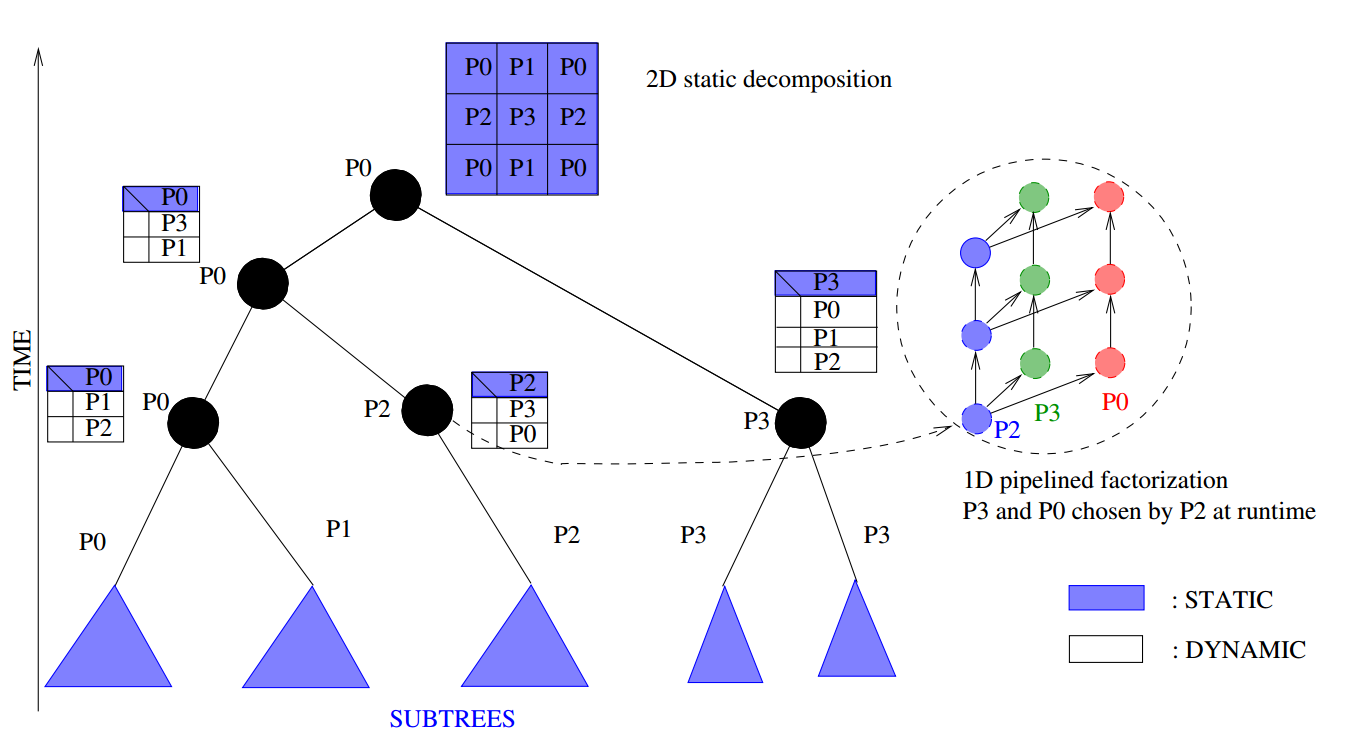
\includegraphics[width=0.55\textwidth]{figures/chapter-2/mumps-task-data-parallelism-2.png}
	\caption{Static and dynamic scheduling in MUMPS, \cite{l2012multifrontal}}
	\label{fig:mumps:mapping-and-scheduling}
\end{figure}

\end{frame}

\subsubsection{Numerical Accuracy}


\begin{frame}[t]{Numerical Accuracy: I}
	\small
	\begin{itemize}
		\item Pivoting is a big issue in direct sparse methods
		\begin{itemize}
			\item analysis: absence of numerical information
			
			\item numerical factorization: it may distort all prediction made during the analysis phases i.e.
			\begin{itemize}
				\item fill-in prediction
				\item load balancing
			\end{itemize}
		\end{itemize}
	\end{itemize}

	\begin{center}
		Therefore, threshold pivoting is commonly used for direct sparse methods
	\end{center}

	Threshold pivoting means that a pivot $|a_{i,i}|$ is accepted if it satisfies:\\
	
	\begin{equation}\label{eq:lc-1}
		|a_{i,i}| \geq \alpha \times max_{k=i \dots n} |a_{k,i}|
	\end{equation}
	
	where $\alpha \in [0,1]$ and $k=i \dots n$ represents row indices of column $i$ within the fully summed block of a frontal matrix.\\
	
\end{frame}



\begin{frame}[t]{Numerical Accuracy: II}
	\small
	\begin{itemize}
		\item In case of small values of $\alpha$
		
		\item solutions can be numerically inaccurate
		\item may demand to perform solution refinements 
	\end{itemize}

	\vspace{5mm}
	As an example, solution accuracy can be improved using:
	\begin{itemize}
		\item  iterative refinement method based a on solution residual
		
		\item  resulting $LU$ decomposition can be used as a preconditioner for a Krylov-based method e.g. GMRES
	\end{itemize}
\end{frame}


% conclusion
\subsection{Conclusion}

%%%%%%%%%%%%%%%%%%%%%%%%%%%%%%%%%%%%%%%%%%%%%%%%%%%%%%%%%%
\begin{frame}[t]{Results and Conclusion}
    \small
    \justifying
    
    \begin{itemize}
	    \item As the first step, various preconditioning algorithms were tested
	    \begin{itemize}
	    	\setlength\itemsep{1mm}
	    	
	    	\item A coarse grid search was used
	    	
	    	\item with maximum 3 values for each tuning parameter 
	    	
	    	\item starting from the default towards more accurate values 
	    	
	    	\item Testing showed there was no preconditioning algorithm 
	    	
	    	\item that could result in convergence for the entire set of matrices 
	    \end{itemize}

	\item Even if we can find an algorithm and suitable parameter settings
	\begin{itemize}
		\setlength\itemsep{1mm}
		
		\item which will result in convergence of the entire matrix set
		
		\item there is no guarantee that it will work in all steps during a simulation
		
		\item Iterative methods cannot fulfill \textit{robustness} criterion
	
	\end{itemize}

	\item Therefore, direct sparse methods is only one way to go
	
	\item In spite of limited tree-task parallelism
\end{itemize}
	 
\end{frame}


%%%%%%%%%%%%%%%%% DSS-LIBS %%%%%%%%%%%%%%
\section{Overview of available Direct Sparse Solver (DSS) libraries}


%%%%%%%%%%%%%%%%%%%%%%%%%%%%%%%%%%%%%%%%%%%%%%%%%%%%%%%%%%
\begin{frame}[t]{List of parallel DSSs}
    \small
    
    \begin{table}[!ht]
    	\footnotesize
    	\centering
    	\begin{tabular}{|c|c|c|c|c|}
    		\hline
    		Package & Method             & Matrix Types                 & \multicolumn{1}{c|}{\begin{tabular}[c]{@{}c@{}}PETSc\\ Interface\end{tabular}} & License      \\ \hline
    		Clique       & Multifrontal       & Symmetric      & \multicolumn{1}{c|}{\begin{tabular}[c]{@{}c@{}}Not \\ Officially\end{tabular}} & Open  \\ \hline
    		MF2          & Multifrontal       & \begin{tabular}[c]{@{}c@{}}Symmetric\\ pattern\end{tabular} & No              & -            \\ \hline
    		DSCPACK      & Multifrontal       & SPD                          & No              & Open \\ \hline
    		MUMPS        & Multifrontal       & General                      & Yes             & Open  \\ \hline
    		PaStiX       & Left looking & General                      & Yes             & Open  \\ \hline
    		PSPASES      & Multifrontal       & SPD                          & No              & Open \\ \hline
    		SPOOLES      & Left-looking       & \begin{tabular}[c]{@{}c@{}}Symmetric\\ pattern\end{tabular} & No              & Open \\ \hline
    		SuperLU\_DIST & Right-looking      & General                      & Yes             & Open  \\ \hline
    		symPACK      & Left-Right looking & SPD                          & No              & Open  \\ \hline
    		S+           & Right-lookin       & General                      & No              & -            \\ \hline
    		
    		PARDISO         & Multifrontal       & General                      & No              & Commercial   \\ \hline
    		
    		WSMP         & Multifrontal       & General                      & No              & Commercial   \\ \hline
    	\end{tabular}
    	\caption{A list of direct sparse linear solvers adapted for \\distributed-memory computations, \cite{list-of-sparse-direct-solvers}, \cite{petsc-web-page}}
    	
    	\label{table:mm-library-spec}
    \end{table}
\end{frame}


\begin{frame}[t]{Comparisons of DSSs}
	\begin{figure}[!h]
		\centering
		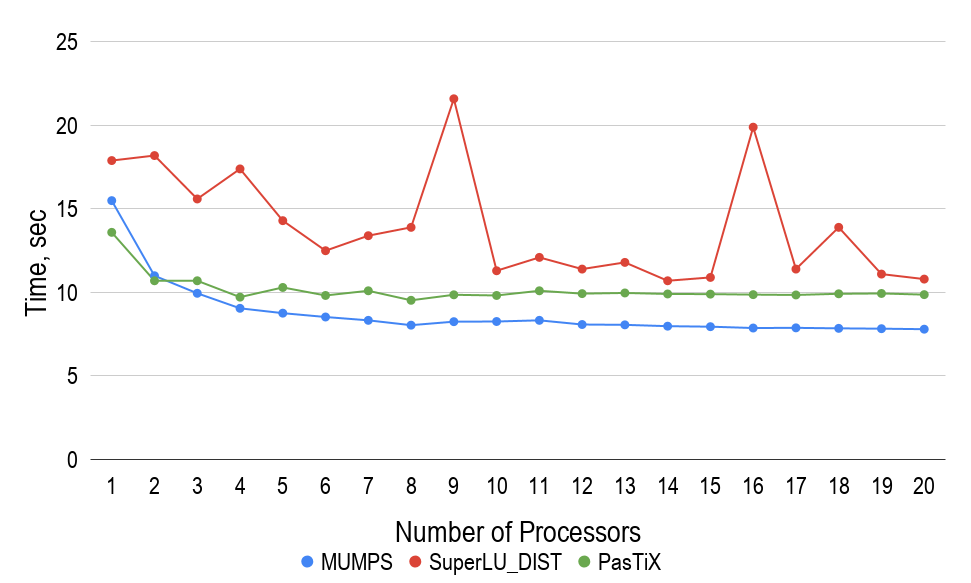
\includegraphics[width=0.875\textwidth]{figures/chapter-2/solvers-comparison-5-point-stencil.png}
		\caption{Comparisons of MUMPS, PasTiX and SuperLU\_DIST libraries during 5 point-stencil Poisson matrix (1000000  equations) factorizations
		}
		\label{fig:5-point-stencil-solvers-comparison}
	\end{figure}
\end{frame}

%%%%%%%%%%%%%%%%% CONFIGURATION %%%%%%%%%%%%%%
\section{Configuration of MUMPS solver
}

\subsection{Overview of MUMPS}

%%%%%%%%%%%%%%%%%%%%%%%%%%%%%%%%%%%%%%%%%%%%%%%%%%%%%%%%%%
\begin{frame}[t]{ABCD}
    \small
    \justifying
    \space
\end{frame}
\subsection{Fill Reducing Reorderings}

%%%%%%%%%%%%%%%%%%%%%%%%%%%%%%%%%%%%%%%%%%%%%%%%%%%%%%%%%%
\begin{frame}[t]{Fill Reducing Reorderings}
	\small
	Sequential:
	\begin{itemize}
		\item Approximate Minimum Degree (AMD) \cite{reordering:AMD}
		
		\item Approximate Minimum Fill (AMF)
		
		\item  Approximate Minimum Degree with automatic quasi-dense row detection (QAMD) \cite{reordering:QAMD}
		
		\item Bottom-up and Top-down Sparse Reordering (PORD) \cite{reordering:PORD}
		
		\item Nested Dissection coupled with AMD (Scotch) \cite{reordering:SCOTCH}
		
		\item Multilevel Nested Dissection coupled with Multiple Minimum Degree (METIS) \cite{reordering:METIS}
	\end{itemize}

	Parallel:
	\begin{itemize}
		\item ParMETIS
		\item PT-Scotch
	\end{itemize}
	
\end{frame}
\subsection{Process pinning}

%%%%%%%%%%%%%%%%%%%%%%%%%%%%%%%%%%%%%%%%%%%%%%%%%%%%%%%%%%
\begin{frame}[t]{Explicit MPI Process Pinnning}
\small
\justifying
To make process pinning \textbf{deterministic}, a python script was developed to automatically generate \textbf{rankfiles} based on the number of \textbf{MPI processes}, \textbf{OpenMP threads} per MPI process, the maximum number of processing elements and the number of \textbf{NUMA domains}.


\begin{figure}
	\centering
	\begin{tabular}{cc}
		\subfloat[Spread]{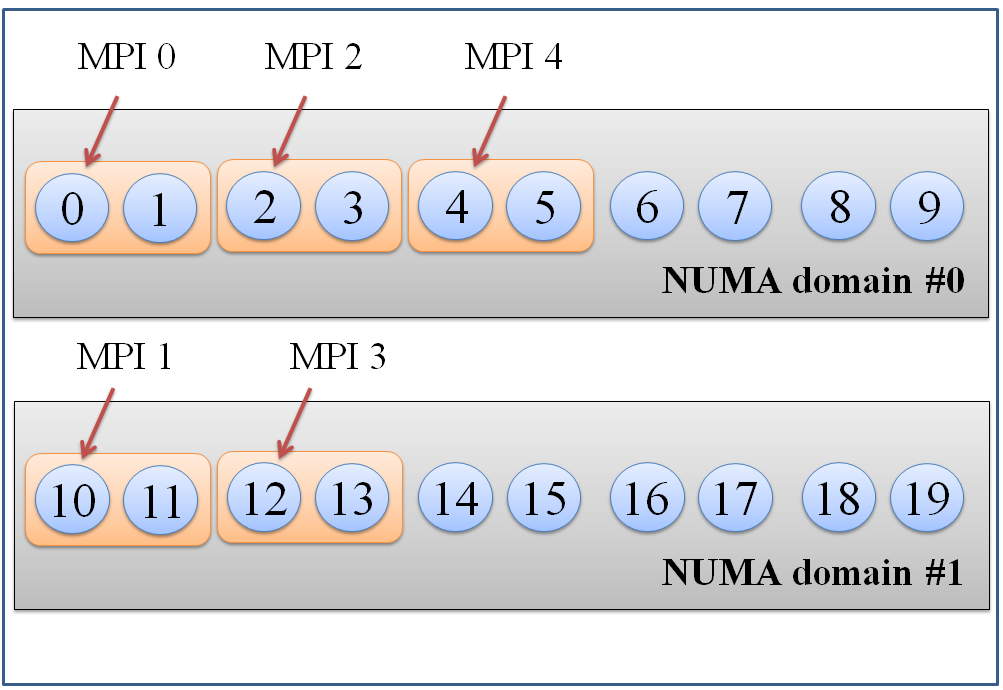
\includegraphics[width=0.4\textwidth]{figures/chapter-2/spread-mode.png} \label{fig:mm-parallel-model-tree-linear}} & 
		\subfloat[Close]{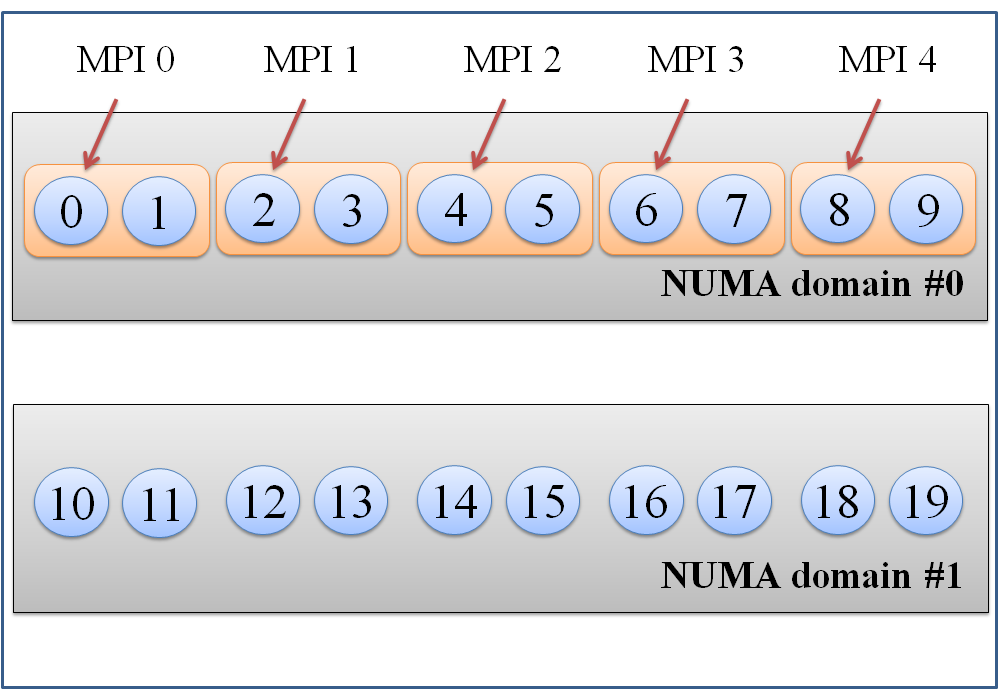
\includegraphics[width=0.4\textwidth]{figures/chapter-2/close-mode.png} \label{fig:mm-parallel-model-tree-quadratic}} \\
	\end{tabular}
	\caption{Process pinning of 2 OpenMP / 1 MPI on HW1 hardware}
	\label{fig:python-script-rankfile-example}
\end{figure}

\end{frame}
\subsection{Configuration of BLAS library}

%%%%%%%%%%%%%%%%%%%%%%%%%%%%%%%%%%%%%%%%%%%%%%%%%%%%%%%%%%
\begin{frame}[t]{ABCD}
    \small
    \justifying
    \space
\end{frame}
\subsection{Hybrid MPI-OpenMP process/thread distribution}

%%%%%%%%%%%%%%%%%%%%%%%%%%%%%%%%%%%%%%%%%%%%%%%%%%%%%%%%%%
\begin{frame}[t]{ABCD}
    \small
    \justifying
    \space
\end{frame}
\subsection{Conclusion}

%%%%%%%%%%%%%%%%%%%%%%%%%%%%%%%%%%%%%%%%%%%%%%%%%%%%%%%%%%
\begin{frame}[t]{ABCD}
    \small
    \justifying
    \space
\end{frame}
\subsection{Recommendations}

%%%%%%%%%%%%%%%%%%%%%%%%%%%%%%%%%%%%%%%%%%%%%%%%%%%%%%%%%%
\begin{frame}[t]{ABCD}
    \small
    \justifying
    \space
\end{frame}


\begin{frame}{Outline II}
    \small
    \tableofcontents[sections={5-7}]
\end{frame}

%%%%%%%%%%%%%%%%%% THEORY %%%%%%%%%%%%%%

\section{Overview of Solver Types}
% Iterative methods
\subsection{Iterative Methods}
\subsubsection{Theory overview}

%%%%%%%%%%%%%%%%%%%%%%%%%%%%%%%%%%%%%%%%%%%%%%%%%%%%%%%%%%
\begin{frame}[t]{Iterative methods}
    \small
    
    \begin{itemize}
    	\item Given an initial guess
    	
    	\item An iterative method generates a sequence of approximate solutions by means of a specific rule
    	
    	\item Depending on a method and the given problem,
    	
    	\item there may exist certain conditions such that the sequence eventually converges to the exact solution
    	
    \end{itemize}

    \begin{itemize}
    	\item There exist two families of iterative methods: \textit{stationary} and \textit{Krylov-based} methods
    	
    	\item Nowadays, Krylov methods dominate in the field of scientific computing
    	
    	\begin{itemize}
    		\item because of their rather fast convergence
    		
    		\item in case of solving well conditioned systems
    		
    		\item or/and a "\textit{good}" initial guess
    	\end{itemize}
    \end{itemize}

\end{frame}


\begin{frame}[t]{Krylov-based methods}
    \small
    \begin{itemize}
    	\item \textit{The key idea} is to construct an approximate solution 
    	\item as a linear combination of vectors $b$, $Ab, \:\: A^2b, \:\: A^3b, \dots A^{n-1}b$
    	\item known as Krylov subspace $\mathcal{K}_{n}$
    	
    	\item where, without of lost of generality, the initial guess $x_0$ is equal to zero
    	
    	\item At each iteration, the subspace is expanded by adding and evaluating the next vector in the sequence
    \end{itemize}

	\begin{itemize}
		\item the methods define and expand another subspace $\mathcal{L}_{n}$ 
		
		\item such that $r_{n} = b - Ax_{n} \perp \mathcal{L}_{n}$ 
		
		\item which is known as the Petrov-Galerkin condition
		
		\item A construction of subspace $\mathcal{L}_{n}$ is defined by a method
		
		\item and based on matrix properties
		
	\end{itemize}
\end{frame}
\subsubsection{Aspects}

%%%%%%%%%%%%%%%%%%%%%%%%%%%%%%%%%%%%%%%%%%%%%%%%%%%%%%%%%%
\ifSpeech
\begin{frame}[t]{Parallelization Aspects: Speech}
    \small
    \justifying
    \begin{itemize}
    	\item Iterative methods usually make use of simple linear algebra kernels e.g. dot products, matrix-vector products, etc.
    	
    	\begin{itemize}
    		\item Therefore, sparsity of linear systems can be handled well
    	\end{itemize}
    	
    	\item The methods make use of data-based parallelism
    	
    	\begin{itemize}
    		\item vectors and matrices are distributed among multiple processing units
    		
    		\item Therefore, the methods scales well in parallel
    		
    		\item the main drop of parallel performance mainly
comes from process-communication overheads	
    	\end{itemize}
    	
    \end{itemize}   
\end{frame}

\begin{frame}[t]{Preconditioners: Speech}
\small
\justifying

\begin{itemize}
	\item In case of a "bad" initial guess $x_{0}$, convergence of iterative methods strongly depends on an involved matrix and, in particular, on its condition number
	
	\item A big condition number usually leads to slow convergence
	
	\item a linear transformation, known as preconditioning, can be applied to the original system of equations
	
	\item to reduce its condition number and, therefore, to accelerate convergence
\end{itemize}

\begin{itemize}
	\item a good preconditioning algorithm should result in
	
	\begin{itemize}
		\item low computational cost
		\item low storage space 
		\item low condition number of the transformed system
		\item adapted for parallel executions as well
	\end{itemize}
\end{itemize}
\end{frame}
\fi


\begin{frame}[t]{Aspects}
\small
\begin{block}{Parallelization Aspects}
	
	\begin{itemize}
		\item Iterative methods usually make use of simple linear algebra kernels e.g. dot products, matrix-vector products, etc.
		
		\item Therefore, the methods efficiently make use of data-based parallelism 
	\end{itemize}
\end{block}

\begin{block}{Numerical Accuracy}
	
	\begin{itemize}
		\item Convergence to the exact solution depends on a value of the  condition number of a matrix
		
		\item Usually requires a linear transformation known as preconditioning
		
		\begin{itemize}
			\item to reduce condition number and accelerate convergence
		\end{itemize}
	\end{itemize}
\end{block}
\end{frame}


\begin{frame}[t]{Preconditioners}
\tiny
\begin{table}[!t]
	\tiny
	\centering
	\begin{tabular}{|c|c|c|c|c|}
		\hline
		\begin{tabular}[c]{@{}c@{}}Package\\ name\end{tabular}     & Origin                                                   & Method                                                        & \begin{tabular}[c]{@{}c@{}}Tuning\\ parameters\end{tabular}                                                                                                                            & Comments                                                                  \\ \hline
		block Jacobi                                               & PETSc                                                    & block Jacobi                                                  & \begin{tabular}[c]{@{}c@{}}-pc\_bjacobi\_blocks\\ -sub\_pc\_type\end{tabular}                                                                                                          & -                                                                         \\ \hline
		\begin{tabular}[c]{@{}c@{}}additive\\ Schwarz\end{tabular} & PETSc                                                    & \begin{tabular}[c]{@{}c@{}}additive\\ Schwarz\end{tabular}    & \begin{tabular}[c]{@{}c@{}}-pc\_asm\_blocks\\ -pc\_asm\_overlap\\ -pc\_asm\_type\\ -pc\_asm\_local\_type\\ -sub\_pc\_type\end{tabular}                                                 & -                                                                         \\ \hline
		euclid                                                     & hypre                                                    & ILU(k)                                                        & \begin{tabular}[c]{@{}c@{}}-nlevel\\ -thresh\\ -filter\end{tabular}                                                                                                                    & \begin{tabular}[c]{@{}c@{}}deprecated\\ form\\ PETSc\end{tabular}         \\ \hline
		pilut                                                      & hypre                                                    & ILU(t)                                                        & \begin{tabular}[c]{@{}c@{}}-pc\_hypre\_pilut\_tol\\ -pc\_hypre\_pilut\_maxiter\\ -pc\_hypre\_pilut\_factorrowsize\end{tabular}                                                         & -                                                                         \\ \hline
		parasail                                                   & hypre                                                    & SPAI                                                          & \begin{tabular}[c]{@{}c@{}}-pc\_hypre\_parasails\_nlevels\\ -pc\_hypre\_parasails\_thresh\\ -pc\_hypre\_parasails\_filter\end{tabular}                                                 & -                                                                         \\ \hline
		SPAI                                                       & \begin{tabular}[c]{@{}c@{}}Grote,\\ Barnard\end{tabular} & SPAI                                                          & \begin{tabular}[c]{@{}c@{}}-pc\_spai\_epsilon\\ -pc\_spai\_nbstep\\ -pc\_spai\_max\\ -pc\_spai\_max\_new\\ -pc\_spai\_block\_size\\ -pc\_spai\_cache\_size\end{tabular}                & -                                                                         \\ \hline
		BoomerAMG                                                  & hypre                                                    & \begin{tabular}[c]{@{}c@{}}algebraic\\ multigrid\end{tabular} & \begin{tabular}[c]{@{}c@{}}-pc\_hypre\_boomeramg\_cycle\_type\\ -pc\_hypre\_boomeramg\_max\_levels\\ -pc\_hypre\_boomeramg\_max\_iter\\ -pc\_hypre\_boomeramg\_tol\\ etc.\end{tabular} & \begin{tabular}[c]{@{}c@{}}39 tuning\\ parameters\\ in total\end{tabular} \\ \hline
	\end{tabular}
	\caption{Parallel preconditioning algorithms available in PETSC}
	\label{table:preconditioners}
\end{table}

\end{frame}






%Direct methods
\subsection{Direct Sparse Methods}
\subsubsection{Theory overview}

%%%%%%%%%%%%%%%%%%%%%%%%%%%%%%%%%%%%%%%%%%%%%%%%%%%%%%%%%%
\begin{frame}[t]{Direct Sparse Methods}
    \small
    \justifying
    
    Direct sparse methods combine the main advantages of direct and iterative methods
    
    \begin{itemize}
    	\item numerical accuracy of the methods is comparable with the standard Gaussian Elimination process
    	
    	\item complexity is bounded by $O(n^{2})$ due to efficient treatment of sparsity
    \end{itemize}

	\vspace{5mm}
	A solution of a system of equations is computed:
	\begin{itemize}
		\item by means of forward and backward substitutions
		 
		\item using $LU$ decomposition of the corresponding matrix.
	\end{itemize}
\end{frame}


\begin{frame}[t]{Direct Sparse Methods: Speech}
	\small
	\justifying
	\begin{itemize}
		\item The multifrontal method is probably the most representative example of direct sparse solvers
		 introduced by Duff and Reid
		 
		 \item The method is an improved version of the frontal method 
		 
		 \item which can compute independent fronts in parallel. 
		 
		 \item A front, also called a frontal matrix, can be considered as a small dense matrix 
		 
		 \item resulting from a column elimination of the original system. 
		 
		 \item There also exist left- and right-looking vatiants of the multifrontal method
		 
	\end{itemize}

	\vspace{5mm}
	Let's consider the multifrontal methods as an example\\
	\vspace{2.5mm}
	To keep the overview rather simple, we assume that matrix $A$ is \textbf{symmetric positive definite} and \textbf{sparse}
	
	
	
\end{frame}


\begin{frame}[t]{Multifrontal Method: I}
	\small
	\justifying
		\begin{equation} \label{eq:chol-1}
		A = LDL^T \qquad \text{with}\quad (D)_{ii} > 0
		\end{equation}
		
		Given a rule and a sparsity pattern, one can build an elimination tree
		\begin{equation} \label{eq:elimination-tree-1}
			p = min(i > j | l_{ij} \neq 0)
		\end{equation}
		
	
	\vspace{-5mm}
		
	\begin{columns}
		\begin{column}{0.5\textwidth}
			\begin{figure}[!htpb]
				\centering
				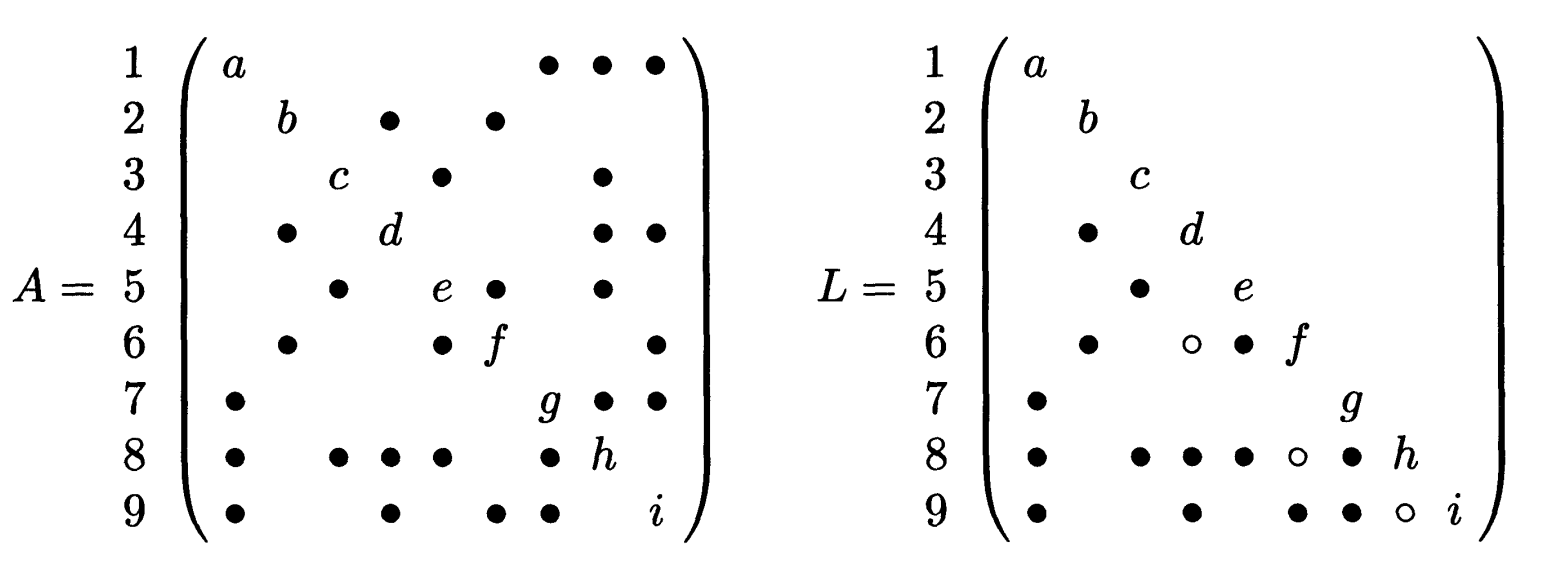
\includegraphics[width=1.2\textwidth]{figures/chapter-2/sparsity-pattern-example-mm.png}
				\caption{A sparse matrix and its Cholesky factor, \cite{mult-frontal-original:2}}
				\label{fig:sparsity-pattern-example-mm}
			\end{figure}
		\end{column}
			
		\begin{column}{0.5\textwidth}
			
			\begin{figure}[!htpb]
				\centering
				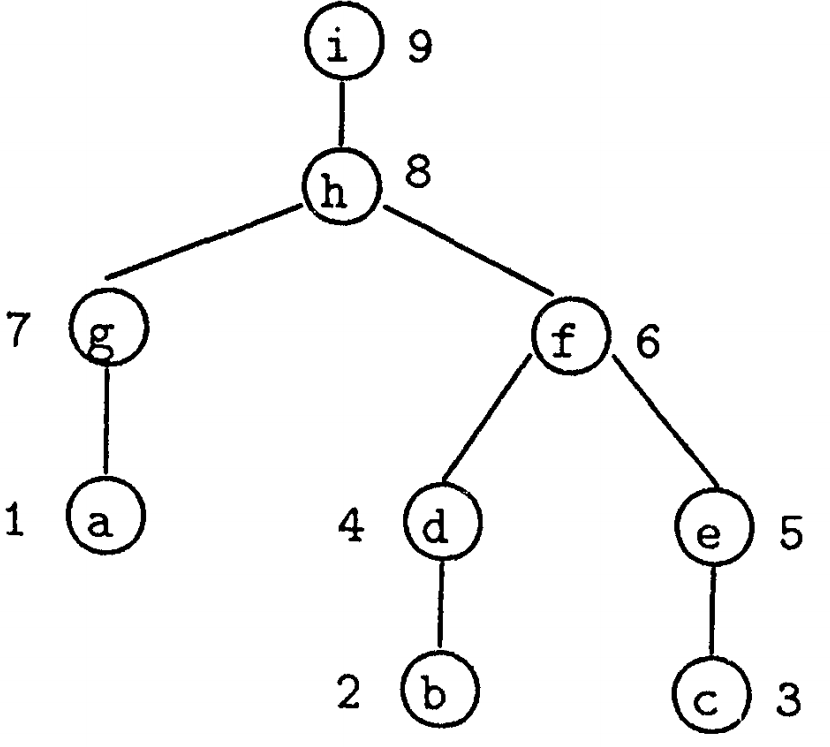
\includegraphics[width=0.65\textwidth]{figures/chapter-2/elimination-tree-mm.png}
				\caption{An elimination tree, \cite{mult-frontal-original:2}}
				\label{fig:elimination-tree-mm}
			\end{figure}
		\end{column}

	\end{columns}
	
	
\end{frame}


\begin{frame}[t]{Multifrontal Method: II}
	\small
	\justifying
	The fundamental idea of the multifrontal method spins around frontal $F$ and update matrices $\hat{U}$
	\begin{equation} \label{eq:mm-1}
		F_{j} = Fr_{j} + \hat{U_{j}} = \begin{bmatrix}a_{j,j} & a_{j,i_1} & a_{j,i_2} & \dots & a_{j,i_r} \\
		a_{i_1,j} \\
		a_{i_2,j} \\
		\vdots & & & 0\\
		a_{i_r,j} \\
		\end{bmatrix} + \hat{U_{j}}
	\end{equation}
	
	where $i_{0}$, $i_{1}$, $i_{2}$, \dots , $i_{r}$ are row subscripts of non-zeros in $L_{*j}$ where $i_{0} = j$; $r$ is the number of off-diagonal non-zero elements.\\


	\begin{equation} \label{eq:mm-2}
		\hat{U_{j}} = - \sum_{k \in T[j] -{j}}  \begin{bmatrix}
		l_{j,k} \\
		l_{i_1,k} \\
		\vdots \\
		l_{i_r,k} \\
		\end{bmatrix} \begin{bmatrix}
		l_{j,k} & l_{i_1,k} & \dots & l_{i_r,k}
		\end{bmatrix} 
	\end{equation}
	
	where $\hat{U_{j}}$ can be treated as the second term of the Schur complement
	
\end{frame}


\begin{frame}[t]{Multifrontal Method: III}
	\small
	\justifying
	Let's consider factorization of a 2-by-2 block matrix $A$
	\begin{equation} \label{eq:mm-3}
		A = \begin{bmatrix}
		B & V^{T} \\
		V & C
		\end{bmatrix} 
		= 
		\begin{bmatrix}
		L_{B} & 0 \\
		VL^{-T}_{B} & I
		\end{bmatrix}
		\begin{bmatrix}
		I & 0 \\
		0 & Sr
		\end{bmatrix} 
		\begin{bmatrix}
		L^{T}_{B} & L^{-1}_{B}V^{T} \\
		0 & I
		\end{bmatrix} 
	\end{equation}
	
	Assuming that block $B$ has already been factorized: $B = L_{B}L^{T}_{B}$\\
	
	\vspace{5mm}
	The Schur complement can be viewed as:
	\begin{equation} \label{eq:mm-3}
	Sr =  C - VB^{-1}V^{T}
	\end{equation}
	
	\begin{columns}
		\begin{column}{0.5\textwidth}
			\textit{Dense Linear Algebra:} $-VB^{-1}V^{T}$\\
			\begin{equation} \label{eq:mm-5}
				-\sum_{k=1}^{j-1}  \begin{bmatrix}
				l_{j,k} \\
				\vdots \\
				l_{n,k} \\
				\end{bmatrix} \begin{bmatrix}
				l_{j,k} & \dots & l_{n,k}
				\end{bmatrix} 
			\end{equation}
		\end{column}
	
		\begin{column}{0.5\textwidth}
			\textit{Multifrontal method:} $\hat{U_{j}}$\\
			\begin{equation} \label{eq:mm-2}
				-\sum_{k \in T[j] -{j}}  \begin{bmatrix}
				l_{i_0,k} \\
				\vdots \\
				l_{i_r,k} \\
				\end{bmatrix} \begin{bmatrix}
				l_{i_0,k} & \dots & l_{i_r,k}
				\end{bmatrix} 
			\end{equation}
		\end{column}
	\end{columns}
	
\end{frame}


\begin{frame}[t]{Multifrontal Method: IV}
	\small
	\justifying
	
	After column $j$ factorization:
	\begin{equation} \label{eq:mm-6}
		\hat{F_{j}} = \begin{bmatrix}
		l_{j,j} & \dots & 0 \\
		\vdots & I \\
		l_{i_{r},j} \\
		\end{bmatrix} 
		\begin{bmatrix}
		1 & \dots & 0 \\
		\vdots & U_{j} \\
		0 \\
		\end{bmatrix} 
		\begin{bmatrix}
		l_{j,j} & \dots & l_{i_{r},j} \\
		\vdots & I \\
		0 \\
		\end{bmatrix} 
	\end{equation}
	where sub-matrix $U_{j}$ represents the full update from all descendants of node $j$ and node $j$ itself
	
	
	\begin{columns}
		
	\begin{column}{0.25\textwidth}
		\begin{figure}[!htpb]
			\centering
			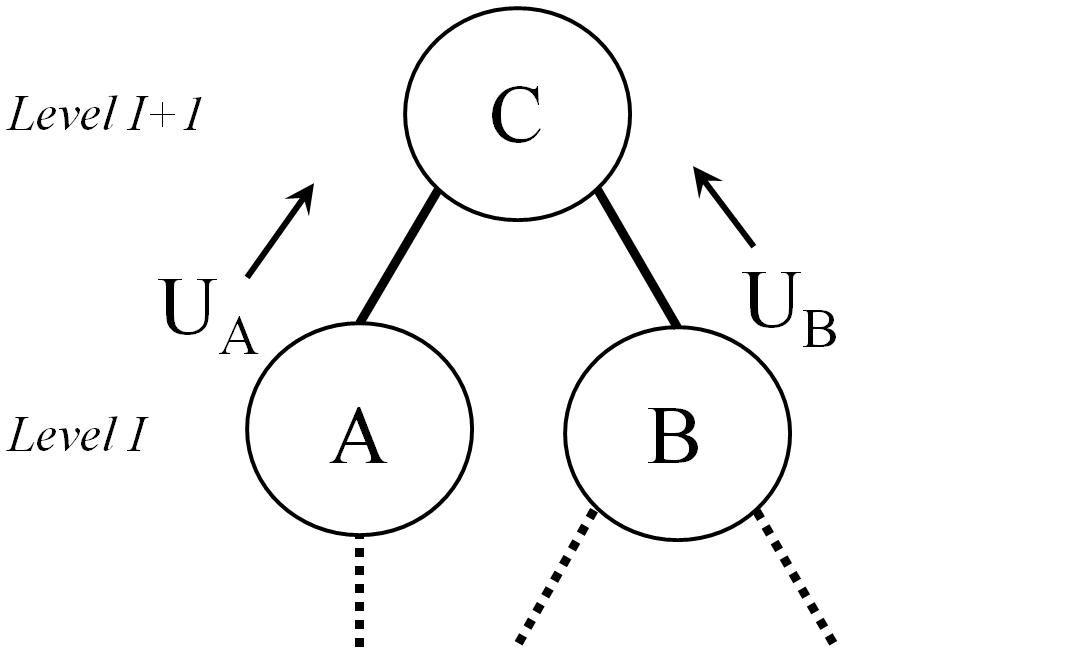
\includegraphics[width=1.35\textwidth]{figures/chapter-2/information-flow.png}
			\caption{Information flow}
			\label{fig:information-float}
		\end{figure}
	\end{column}

	\begin{column}{0.75\textwidth}
		\begin{equation} \label{eq:mm-9}
			F_{j} = \begin{bmatrix}a_{j,j} & a_{j,i_1} & a_{j,i_2} & \dots & a_{j,i_r} \\
			a_{i_1,j} \\
			a_{i_1,j} \\
			\vdots & & & 0\\
			a_{i_r,j} \\
			\end{bmatrix} \extendadd U_{c_1} \extendadd \dots \extendadd U_{c_s} 
		\end{equation}
	\end{column}

	\end{columns}
\end{frame}



\begin{frame}[t]{Supernodal Method}
	\small
	
	\begin{itemize}
		\item In practice, an improved version of the multifrontal method is used
		\item A super-node is formed by a set of contiguous columns 
		
		\item which have the same  off-diagonal sparsity structure
	\end{itemize}

	\begin{equation} \label{eq:mm-10}
		\mathcal{F}_{j} = \begin{bmatrix}a_{j,j} & a_{j,j+1} & \dots & a_{j,j+t}  & a_{j,i_1} & \dots & a_{j,i_r} \\
		a_{j+1,j} & a_{j+1,j+1} & \dots & a_{j+1,j+t}  & a_{j+1,i_1} & \dots & a_{j+1,i_r} \\
		\vdots & \vdots & \dots & \vdots \\
		a_{j+t,j}  & a_{j+t,j+1} & \dots & a_{j+t,j+t}  & a_{j+t,i_1} & \dots & a_{j+t,i_r} \\
		a_{i_1,j} & a_{i_1,j+1} & \dots & a_{i_1,j+t} \\
		\vdots & \vdots & \dots & \vdots  & & 0\\ 
		a_{i_r,j} & a_{i_r,j+1} & \dots & a_{i_r,j+t} \\
		\end{bmatrix} \extendadd U_{c_1} \dots \extendadd U_{c_s} 
	\end{equation}

\end{frame}
\subsubsection{Parallelization Aspects}

%%%%%%%%%%%%%%%%%%%%%%%%%%%%%%%%%%%%%%%%%%%%%%%%%%%%%%%%%%

\begin{frame}[t]{Parallelization Aspects}
\small

\vspace{-5mm}
\begin{columns}
	\begin{column}{0.5\textwidth}
		\begin{figure}
			\centering
			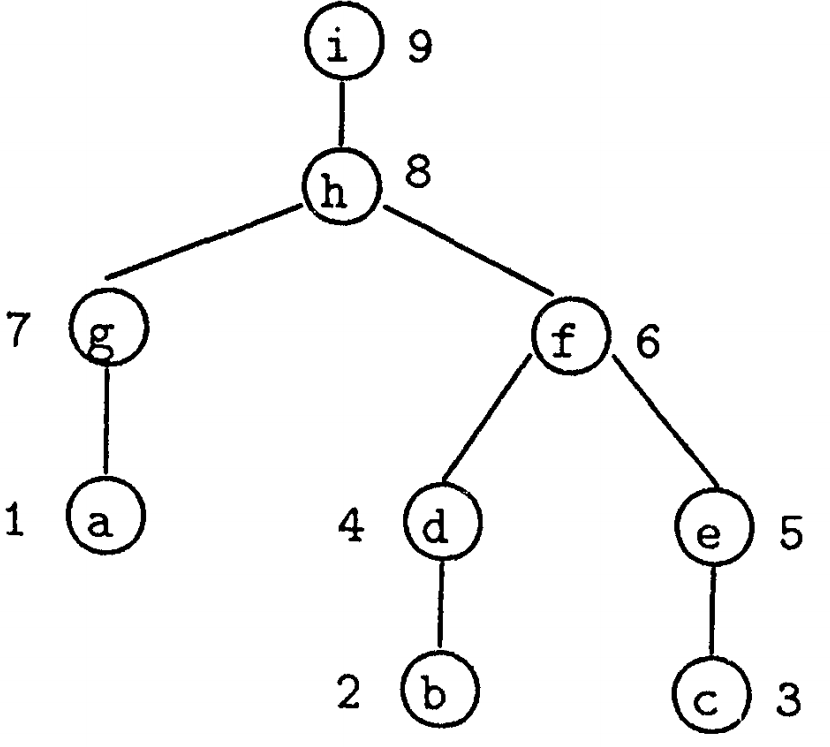
\includegraphics[width=0.3\textheight]{figures/chapter-2/elimination-tree-mm.png}
			\caption{Original elimination tree}
		\end{figure}
	\end{column}
	
	\begin{column}{0.5\textwidth}
		\begin{figure}
			\centering
			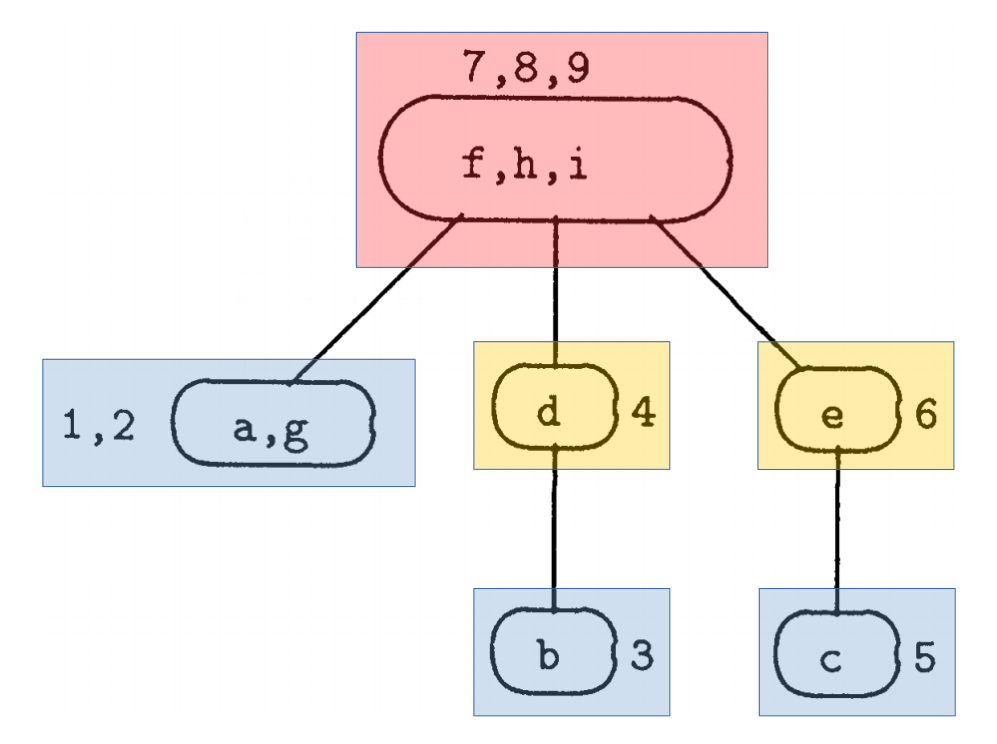
\includegraphics[width=0.6\textwidth]{figures/chapter-2/elimination-tree-parallel.png}
			\caption{Supernodal/assembly tree}
		\end{figure}
	\end{column}
	
\end{columns}

\begin{figure}[!htpb]
	\centering
	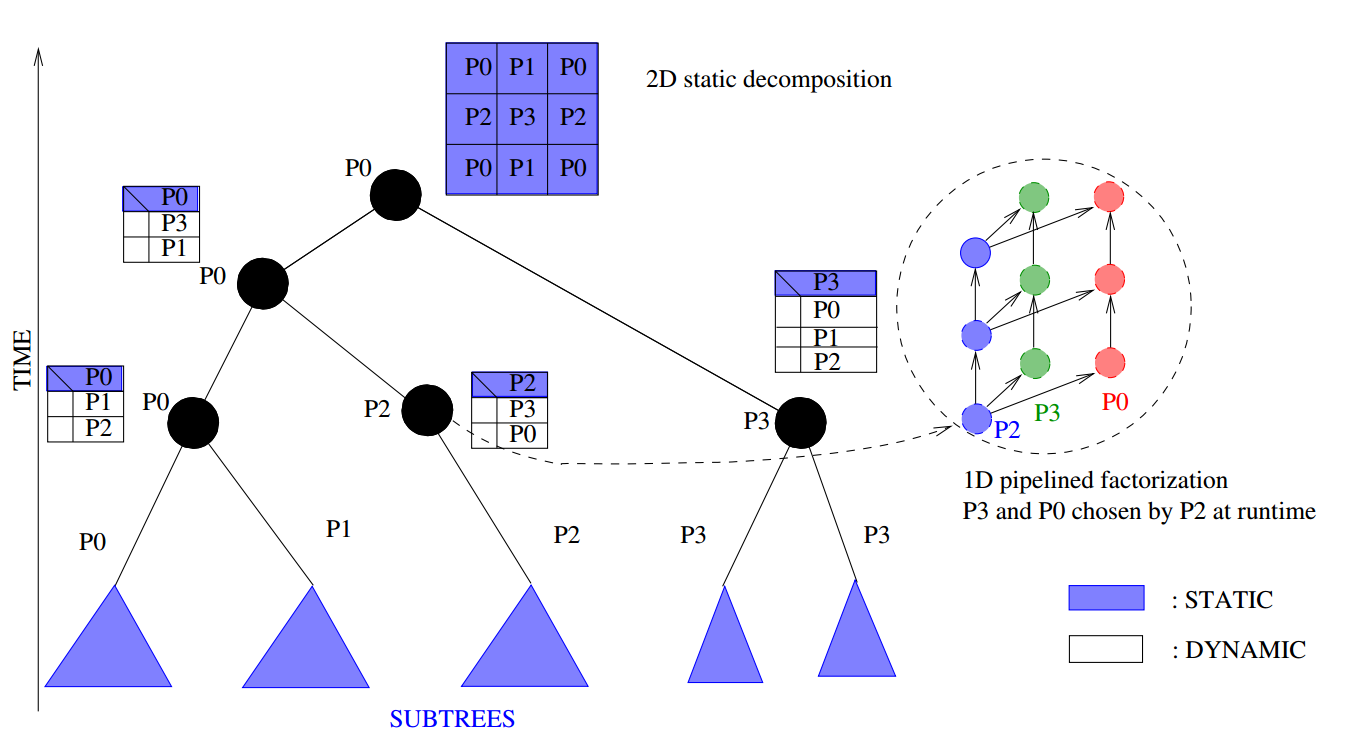
\includegraphics[width=0.55\textwidth]{figures/chapter-2/mumps-task-data-parallelism-2.png}
	\caption{Static and dynamic scheduling in MUMPS, \cite{l2012multifrontal}}
	\label{fig:mumps:mapping-and-scheduling}
\end{figure}

\end{frame}

\subsubsection{Numerical Accuracy}


\begin{frame}[t]{Numerical Accuracy: I}
	\small
	\begin{itemize}
		\item Pivoting is a big issue in direct sparse methods
		\begin{itemize}
			\item analysis: absence of numerical information
			
			\item numerical factorization: it may distort all prediction made during the analysis phases i.e.
			\begin{itemize}
				\item fill-in prediction
				\item load balancing
			\end{itemize}
		\end{itemize}
	\end{itemize}

	\begin{center}
		Therefore, threshold pivoting is commonly used for direct sparse methods
	\end{center}

	Threshold pivoting means that a pivot $|a_{i,i}|$ is accepted if it satisfies:\\
	
	\begin{equation}\label{eq:lc-1}
		|a_{i,i}| \geq \alpha \times max_{k=i \dots n} |a_{k,i}|
	\end{equation}
	
	where $\alpha \in [0,1]$ and $k=i \dots n$ represents row indices of column $i$ within the fully summed block of a frontal matrix.\\
	
\end{frame}



\begin{frame}[t]{Numerical Accuracy: II}
	\small
	\begin{itemize}
		\item In case of small values of $\alpha$
		
		\item solutions can be numerically inaccurate
		\item may demand to perform solution refinements 
	\end{itemize}

	\vspace{5mm}
	As an example, solution accuracy can be improved using:
	\begin{itemize}
		\item  iterative refinement method based a on solution residual
		
		\item  resulting $LU$ decomposition can be used as a preconditioner for a Krylov-based method e.g. GMRES
	\end{itemize}
\end{frame}


% conclusion
\subsection{Conclusion}

%%%%%%%%%%%%%%%%%%%%%%%%%%%%%%%%%%%%%%%%%%%%%%%%%%%%%%%%%%
\begin{frame}[t]{Results and Conclusion}
    \small
    \justifying
    
    \begin{itemize}
	    \item As the first step, various preconditioning algorithms were tested
	    \begin{itemize}
	    	\setlength\itemsep{1mm}
	    	
	    	\item A coarse grid search was used
	    	
	    	\item with maximum 3 values for each tuning parameter 
	    	
	    	\item starting from the default towards more accurate values 
	    	
	    	\item Testing showed there was no preconditioning algorithm 
	    	
	    	\item that could result in convergence for the entire set of matrices 
	    \end{itemize}

	\item Even if we can find an algorithm and suitable parameter settings
	\begin{itemize}
		\setlength\itemsep{1mm}
		
		\item which will result in convergence of the entire matrix set
		
		\item there is no guarantee that it will work in all steps during a simulation
		
		\item Iterative methods cannot fulfill \textit{robustness} criterion
	
	\end{itemize}

	\item Therefore, direct sparse methods is only one way to go
	
	\item In spite of limited tree-task parallelism
\end{itemize}
	 
\end{frame}


%%%%%%%%%%%%%%%%% DSS-LIBS %%%%%%%%%%%%%%
\section{Overview of available Direct Sparse Solver (DSS) libraries}


%%%%%%%%%%%%%%%%%%%%%%%%%%%%%%%%%%%%%%%%%%%%%%%%%%%%%%%%%%
\begin{frame}[t]{List of parallel DSSs}
    \small
    
    \begin{table}[!ht]
    	\footnotesize
    	\centering
    	\begin{tabular}{|c|c|c|c|c|}
    		\hline
    		Package & Method             & Matrix Types                 & \multicolumn{1}{c|}{\begin{tabular}[c]{@{}c@{}}PETSc\\ Interface\end{tabular}} & License      \\ \hline
    		Clique       & Multifrontal       & Symmetric      & \multicolumn{1}{c|}{\begin{tabular}[c]{@{}c@{}}Not \\ Officially\end{tabular}} & Open  \\ \hline
    		MF2          & Multifrontal       & \begin{tabular}[c]{@{}c@{}}Symmetric\\ pattern\end{tabular} & No              & -            \\ \hline
    		DSCPACK      & Multifrontal       & SPD                          & No              & Open \\ \hline
    		MUMPS        & Multifrontal       & General                      & Yes             & Open  \\ \hline
    		PaStiX       & Left looking & General                      & Yes             & Open  \\ \hline
    		PSPASES      & Multifrontal       & SPD                          & No              & Open \\ \hline
    		SPOOLES      & Left-looking       & \begin{tabular}[c]{@{}c@{}}Symmetric\\ pattern\end{tabular} & No              & Open \\ \hline
    		SuperLU\_DIST & Right-looking      & General                      & Yes             & Open  \\ \hline
    		symPACK      & Left-Right looking & SPD                          & No              & Open  \\ \hline
    		S+           & Right-lookin       & General                      & No              & -            \\ \hline
    		
    		PARDISO         & Multifrontal       & General                      & No              & Commercial   \\ \hline
    		
    		WSMP         & Multifrontal       & General                      & No              & Commercial   \\ \hline
    	\end{tabular}
    	\caption{A list of direct sparse linear solvers adapted for \\distributed-memory computations, \cite{list-of-sparse-direct-solvers}, \cite{petsc-web-page}}
    	
    	\label{table:mm-library-spec}
    \end{table}
\end{frame}


\begin{frame}[t]{Comparisons of DSSs}
	\begin{figure}[!h]
		\centering
		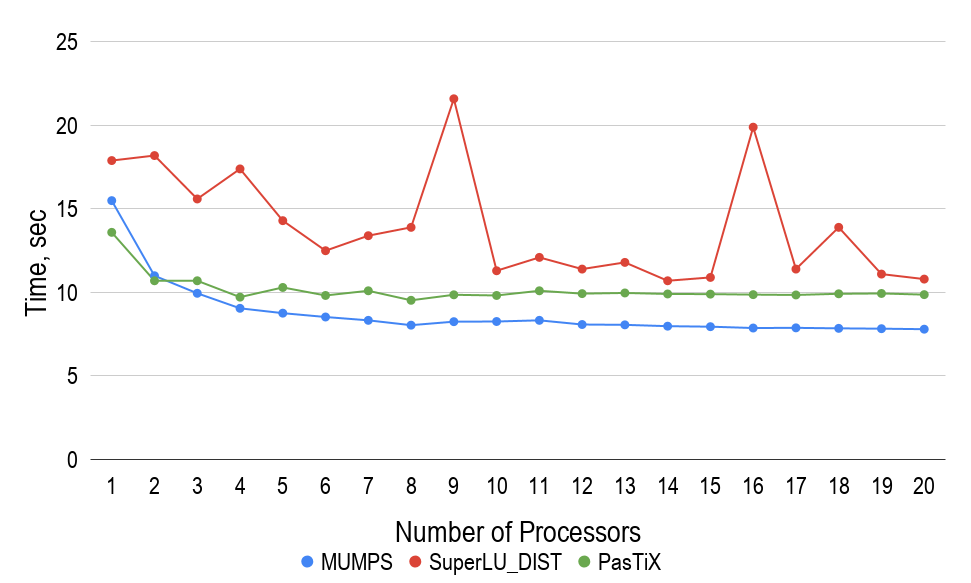
\includegraphics[width=0.875\textwidth]{figures/chapter-2/solvers-comparison-5-point-stencil.png}
		\caption{Comparisons of MUMPS, PasTiX and SuperLU\_DIST libraries during 5 point-stencil Poisson matrix (1000000  equations) factorizations
		}
		\label{fig:5-point-stencil-solvers-comparison}
	\end{figure}
\end{frame}

%%%%%%%%%%%%%%%%% CONFIGURATION %%%%%%%%%%%%%%
\section{Configuration of MUMPS solver
}

\subsection{Overview of MUMPS}

%%%%%%%%%%%%%%%%%%%%%%%%%%%%%%%%%%%%%%%%%%%%%%%%%%%%%%%%%%
\begin{frame}[t]{ABCD}
    \small
    \justifying
    \space
\end{frame}
\subsection{Fill Reducing Reorderings}

%%%%%%%%%%%%%%%%%%%%%%%%%%%%%%%%%%%%%%%%%%%%%%%%%%%%%%%%%%
\begin{frame}[t]{Fill Reducing Reorderings}
	\small
	Sequential:
	\begin{itemize}
		\item Approximate Minimum Degree (AMD) \cite{reordering:AMD}
		
		\item Approximate Minimum Fill (AMF)
		
		\item  Approximate Minimum Degree with automatic quasi-dense row detection (QAMD) \cite{reordering:QAMD}
		
		\item Bottom-up and Top-down Sparse Reordering (PORD) \cite{reordering:PORD}
		
		\item Nested Dissection coupled with AMD (Scotch) \cite{reordering:SCOTCH}
		
		\item Multilevel Nested Dissection coupled with Multiple Minimum Degree (METIS) \cite{reordering:METIS}
	\end{itemize}

	Parallel:
	\begin{itemize}
		\item ParMETIS
		\item PT-Scotch
	\end{itemize}
	
\end{frame}
\subsection{Process pinning}

%%%%%%%%%%%%%%%%%%%%%%%%%%%%%%%%%%%%%%%%%%%%%%%%%%%%%%%%%%
\begin{frame}[t]{Explicit MPI Process Pinnning}
\small
\justifying
To make process pinning \textbf{deterministic}, a python script was developed to automatically generate \textbf{rankfiles} based on the number of \textbf{MPI processes}, \textbf{OpenMP threads} per MPI process, the maximum number of processing elements and the number of \textbf{NUMA domains}.


\begin{figure}
	\centering
	\begin{tabular}{cc}
		\subfloat[Spread]{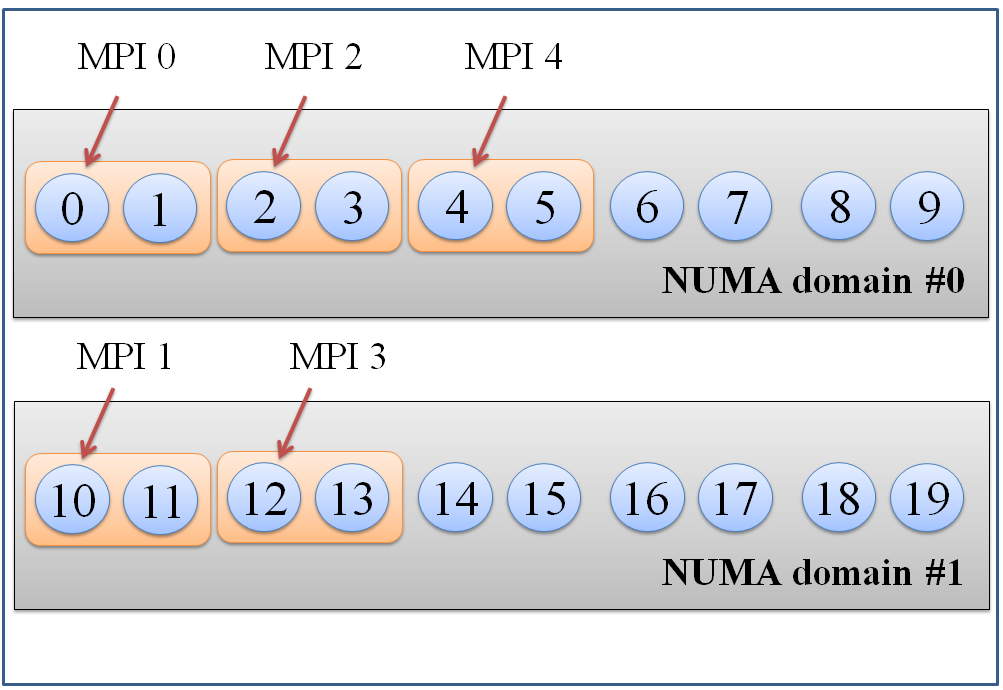
\includegraphics[width=0.4\textwidth]{figures/chapter-2/spread-mode.png} \label{fig:mm-parallel-model-tree-linear}} & 
		\subfloat[Close]{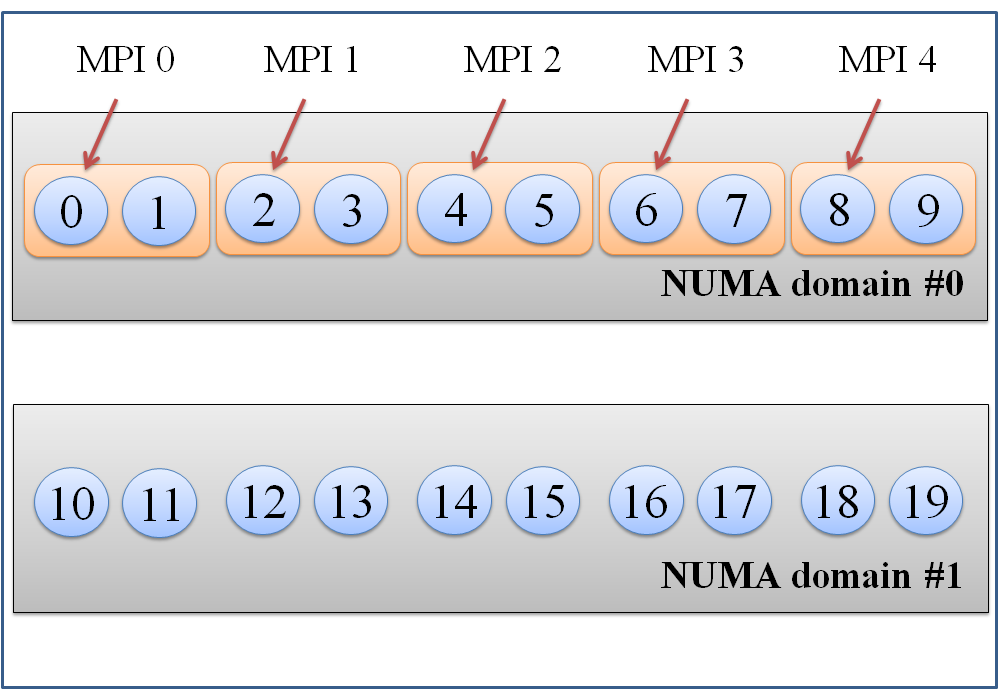
\includegraphics[width=0.4\textwidth]{figures/chapter-2/close-mode.png} \label{fig:mm-parallel-model-tree-quadratic}} \\
	\end{tabular}
	\caption{Process pinning of 2 OpenMP / 1 MPI on HW1 hardware}
	\label{fig:python-script-rankfile-example}
\end{figure}

\end{frame}
\subsection{Configuration of BLAS library}

%%%%%%%%%%%%%%%%%%%%%%%%%%%%%%%%%%%%%%%%%%%%%%%%%%%%%%%%%%
\begin{frame}[t]{ABCD}
    \small
    \justifying
    \space
\end{frame}
\subsection{Hybrid MPI-OpenMP process/thread distribution}

%%%%%%%%%%%%%%%%%%%%%%%%%%%%%%%%%%%%%%%%%%%%%%%%%%%%%%%%%%
\begin{frame}[t]{ABCD}
    \small
    \justifying
    \space
\end{frame}
\subsection{Conclusion}

%%%%%%%%%%%%%%%%%%%%%%%%%%%%%%%%%%%%%%%%%%%%%%%%%%%%%%%%%%
\begin{frame}[t]{ABCD}
    \small
    \justifying
    \space
\end{frame}
\subsection{Recommendations}

%%%%%%%%%%%%%%%%%%%%%%%%%%%%%%%%%%%%%%%%%%%%%%%%%%%%%%%%%%
\begin{frame}[t]{ABCD}
    \small
    \justifying
    \space
\end{frame}





%%%%%%%%%%%%%%%%%%%% TASK 2 %%%%%%%%%%%%%%%%%%%%
%\section{Improvement of ATHLET-NuT communication}
\subsection{Overview of Jacobian matrix compression algorithm}


%%%%%%%%%%%%%%%%%%%%%%%%%%%%%%%%%%%%%%%%%%%%%%%%%%%%%%%%%%
\begin{frame}[t]{Jacobian Matrix Approximation}
    \spc
    \justifying
    %\small
    
    In the general case, \textbf{finite difference} method can be used to compute a \textbf{Jacobian} matrix \textbf{approximation} in the following way:
    
    \begin{equation} \label{eq:matrix-compression-1}
	    \frac{1}{\epsilon} (F(y + \epsilon e_{k}) - F(y)) \approx J(y) e_{k}, \: \: \: 1 \leq k \leq N
    \end{equation}

    where $F : \mathbb{R}^{N} \rightarrow \mathbb{R}^{N}$  is a non-linear function, $e_{k} \in \mathbb{R}^{N}$ is the k\textit{th}  \textbf{coordinate} unit \textbf{vector}, $\epsilon$ is a small step size.\\
    
    \begin{block}{Drawbacks:}
        \begin{itemize}
            \item Matrix sparsity is not exploited
            \item Requires $N$ function evaluations
        \end{itemize}
    \end{block}
    
\end{frame}

\ifSpeech
%%%%%%%%%%%%%%%%%%%%%%%%%%%%%%%%%%%%%%%%%%%%%%%%%%%%%%%%%%
\begin{frame}[t]{Compression, Matrix Partitioning}
    \justifying
    \small
    
    Compression is based on the notion of \textbf{structurally orthogonal} columns\\ 
    i.e. \underline{columns which do not share any non-zero entry in a common row}.
    
    \spc
        
    \textbf{Example:}
        \begin{itemize}
            \item Instead of using 5 coordinate unit vectors $e_{k}$, where $1 \leq k \leq 5 $  
            \item The same Jacobian can be approximated with \textbf{3 seed vectors} $d$: $d_{1} = [1,0,1,0,0]^{T}$, $d_{2} = [0,1,0,0,0]^{T}$, $d_{3} = [0,0,1,0,1]^{T}$
    \end{itemize}

        
    \begin{figure}[htpb]
        \centering
        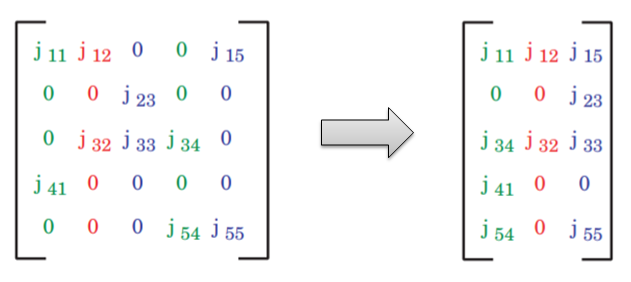
\includegraphics[width=0.50\textwidth]{figures/chapter-3/matrix-compression-example.png}
        \caption{An example of matrix coloring and compression \cite{gebremedhin2005color}}
        \label{fig:example-of-matrix-compression}
    \end{figure}
    

\end{frame}
\fi

%%%%%%%%%%%%%%%%%%%%%%%%%%%%%%%%%%%%%%%%%%%%%%%%%%%%%%%%%%
\begin{frame}[t]{Seeding, Partitioning, Compression}
    \justifying
    \small
    
    \begin{itemize}
        \item Seeding/Partitioning is based on \textbf{structurally orthogonal} columns i.e. columns which do not share any non-zero entry in a common row
    
        \item \textbf{efficiency} \textbf{requires} partitioning into \textbf{the fewest amount of} groups, \textbf{colors}, because evaluation of $F(y + \delta)$ is expensive
    \end{itemize}

    \begin{equation}
	    \frac{1}{\epsilon} (F(y + \epsilon d_{i}) - F(y)) \approx J(y) d_{i}, \: \: \: 1 \leq i \leq c << N
    \end{equation}
    
    \begin{figure}[htpb]
    \centering
    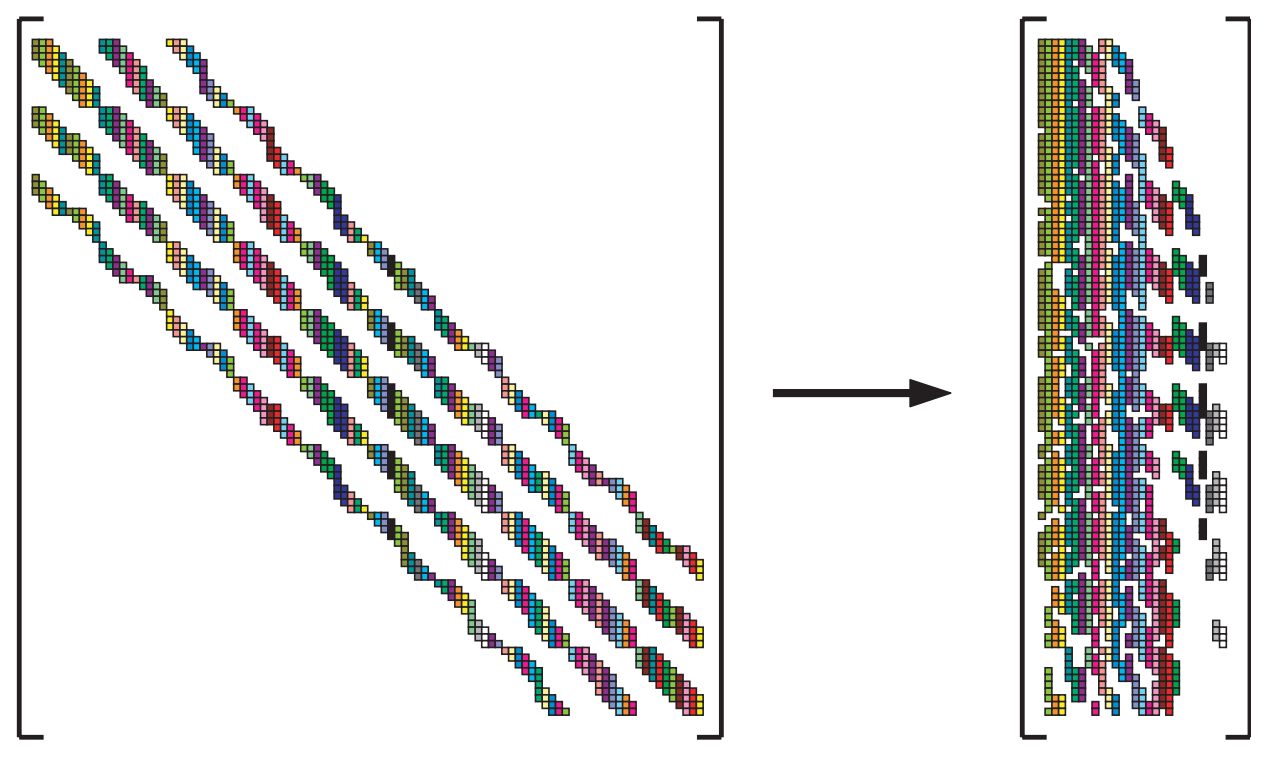
\includegraphics[width=0.5\textwidth]{figures/matrix-compression.png}
    \caption{An example of Jacobian matrix partitioning     \cite{gebremedhin2005color}}
    \end{figure}

\end{frame}


%%%%%%%%%%%%%%%%%%%%%%%%%%%%%%%%%%%%%%%%%%%%%%%%%%%%%%%%%%
\begin{frame}[t]{Arisen Problem due to ATHLET-NuT Design}
    \justifying
    \footnotesize

        \begin{itemize}
            \item Column vector \textbf{length} of the compressed Jacobian form is gradually \textbf{decreasing}
            
            \item Column length \textbf{distribution defines} the \textbf{communication pattern} between ATHLET and NuT
            
            \item Each \textbf{column transfer} is a service and, thus, it goes through \textbf{synchronous 3-way handshake} communication
            
        \end{itemize}


    \begin{columns}
    \column{0.7\textwidth}
        \begin{figure}[t]
            \centering
            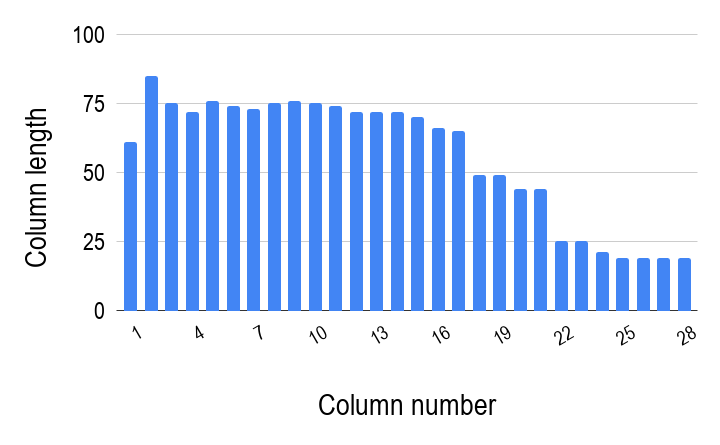
\includegraphics[width=0.9\textwidth]{figures/matrix-compression-2.png}
        \end{figure}
    \column{0.3\textwidth}
        \begin{figure}[t]
            \centering
            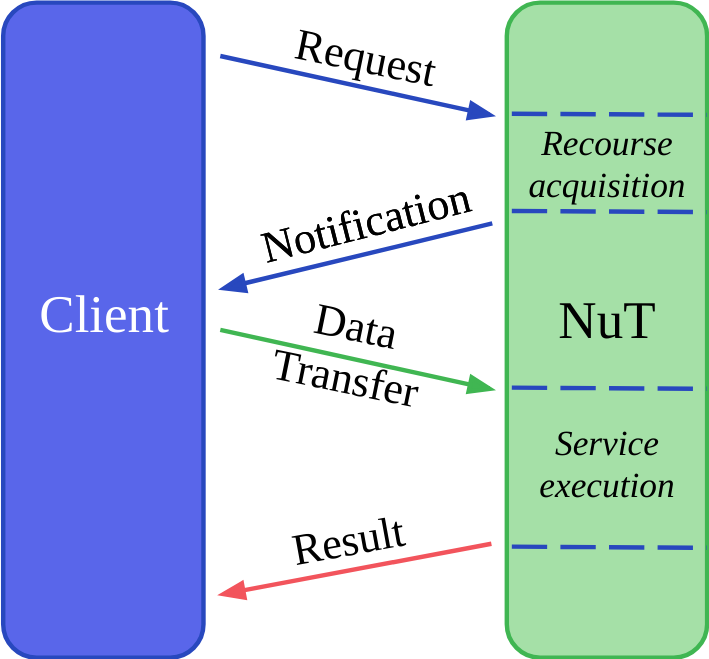
\includegraphics[width=0.9\textwidth]{figures/presentation-figures/handshake.png}
        \end{figure}
    \end{columns}

\end{frame}
\subsection{Accumulator Concept}

\ifCommentInclude
%%%%%%%%%%%%%%%%%%%%%%%%%%%%%%%%%%%%%%%%%%%%%%%%%%%%%%%%%%
\begin{frame}[t]{Accumulator Concept}
    \justifying
    
    \begin{figure}[htpb]
        \centering
        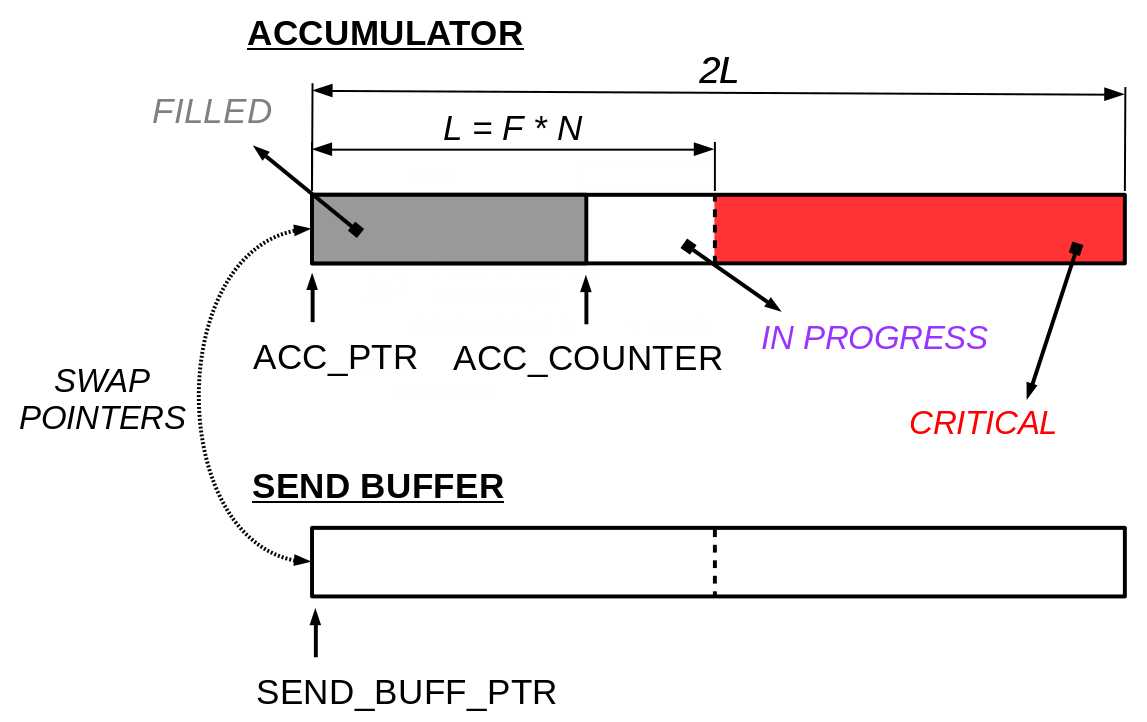
\includegraphics[width=0.8\textwidth]{figures/chapter-3/accumulator-concept.png}
        \caption{Accumulator concept} \label{fig:accumulator-concept}
    \end{figure}

\end{frame}
\fi

%%%%%%%%%%%%%%%%%%%%%%%%%%%%%%%%%%%%%%%%%%%%%%%%%%%%%%%%%%
\begin{frame}[t]{Accumulator Concept}
    \justifying
    \begin{columns}
    \column{0.5\textwidth}
        \begin{figure}[t]
            \centering
            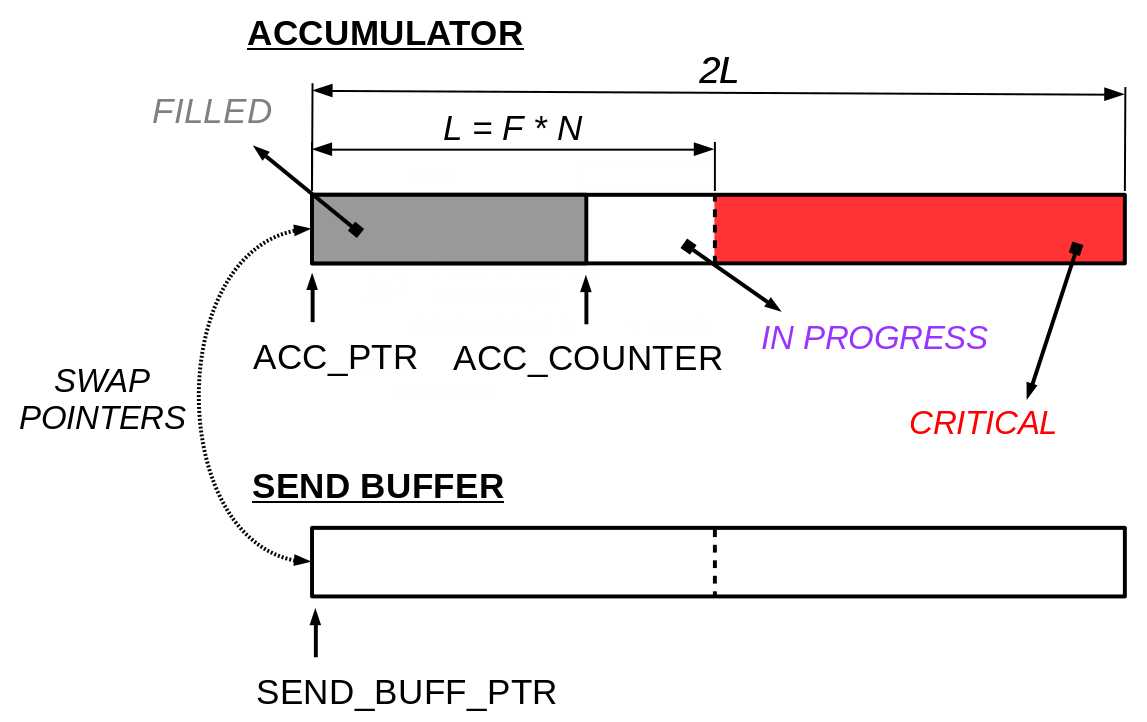
\includegraphics[width=0.9\textwidth]{figures/chapter-3/accumulator-concept.png}
        \end{figure}
    \column{0.5\textwidth}
        \begin{figure}[t]
            \centering
            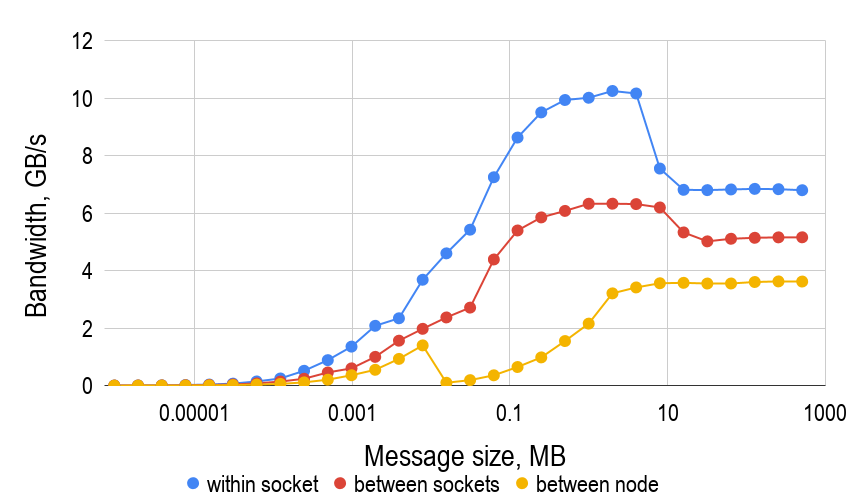
\includegraphics[width=0.9\textwidth]{figures/chapter-3/hw1-bandwidth.png} \label{fig:hw1-bandwidth}
        \end{figure}
    \end{columns}
    
    \spc
    Accumulator concept allows to:
    \begin{itemize}
        \item enable \textbf{non-blocking} data transfer
        \item \textbf{reduce} the number of client \textbf{requests} i.e. handshakes, resource acquisitions
        \item achieve \textbf{full bandwidth} utilization
        
    \end{itemize}

\end{frame}

%%%%%%%%%%%%%%%%%%%%%%%%%%%%%%%%%%%%%%%%%%%%%%%%%%%%%%%%%%
\begin{frame}[t]{Example:  N = 100; F = 1}
    \small
    \justifying
    \begin{itemize}
        \item The original \textbf{distribution shape} is transformed to the \textbf{rectangular} one
        \item Data is transferred in \textbf{equal chunks}
    \end{itemize}
    
    
    \begin{figure}[t]
        \centering
	    \begin{tabular}{cc}
		    \subfloat[Before]{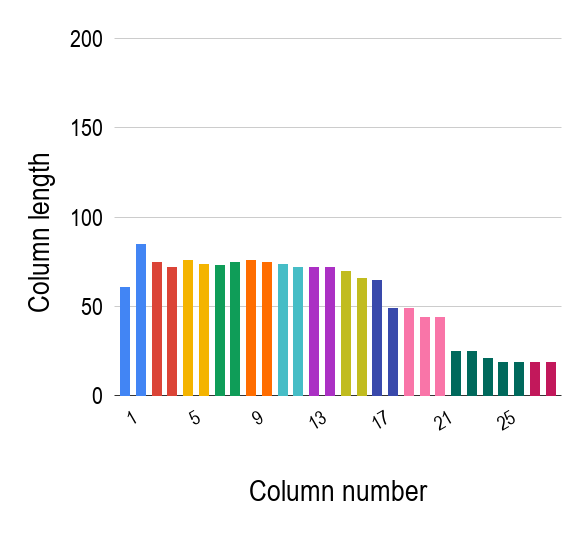
\includegraphics[width=0.42\textwidth]{figures/chapter-3/accumulation-before.png}} &
		    \subfloat[After]{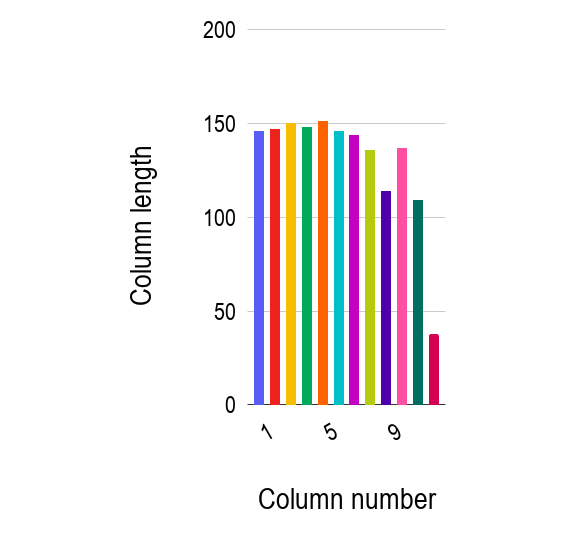
\includegraphics[width=0.42\textwidth]{figures/chapter-3/accumulation-after.png}} \\
	        \end{tabular}
	\label{fig:accumulator-in-action}
    \end{figure}

\end{frame}
\subsection{Benchmarks and Test Data}

\ifPresentation
%%%%%%%%%%%%%%%%%%%%%%%%%%%%%%%%%%%%%%%%%%%%%%%%%%%%%%%%%%
\begin{frame}[t]{Benchmarks}

    \justifying
    
    \begin{itemize}
        \setlength\itemsep{0.5cm}
        
        \item \textbf{Testing} of new concepts and ideas directly \text{in ATHLET} can be quite:
        \begin{itemize}
            \item cumbersome
            \item computationally expensive
            \item inconvenient
        \end{itemize}
        
        \item Therefore, two dedicated benchmarks have been developed:
            \begin{enumerate}
                \item \textbf{BM1}: tests \textbf{only} data \textbf{accumulation} i.e. uses \textbf{MPI\_Bcast}
                
                \item \textbf{BM2}: tests \textbf{both} data accumulation and non-blocking data transfer i.e. uses \textbf{MPI\_Ibcast}
            \end{enumerate}
            
        \item The benchmarks fully replicates all \textbf{basic ideas} of ATHLET
        
        \item Column vectors are generated \textbf{without} compute-expensive \textbf{function evaluations} i.e. filled with random numbers
    \end{itemize}

\end{frame}


%%%%%%%%%%%%%%%%%%%%%%%%%%%%%%%%%%%%%%%%%%%%%%%%%%%%%%%%%%
\begin{frame}[t]{Test Data and Process Allocation}

    \justifying
    \small
   
     \begin{figure}[t]
        \centering
        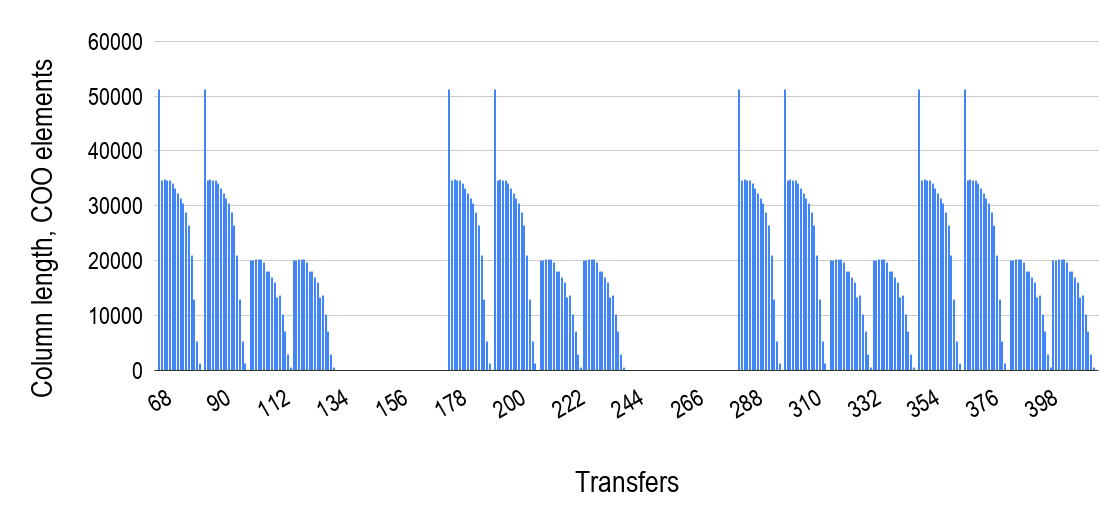
\includegraphics[width=0.6\textwidth]{figures/chapter-3/communication-pattern.png}
        \caption{A part of \textbf{cube-64} communication pattern}
    \end{figure}

    \vspace{-20.0pt}
    \begin{itemize}
        \item \textbf{Patterns} of the most common GRS simulations were \textbf{recorded}
    
        \item The recordings were \textbf{played inside} of the benchmarks
    
        \item The recordings were used \textbf{to generate} dummy column arrays
    
        \item Tested for \textbf{intra-socket, intra-node and inter-node} communication
    
    \end{itemize}

\end{frame}
\fi

\ifSpeech
%%%%%%%%%%%%%%%%%%%%%%%%%%%%%%%%%%%%%%%%%%%%%%%%%%%%%%%%%%
\begin{frame}[t]{Test Data}
    \justifying
    \begin{itemize}
        \item Communication \textbf{patterns were recorded} while ATHEL was executing some common GRS simulations
        
        \item The recordings were used \textbf{to generate} the corresponding column vector \textbf{lengths}
        
        \item The recordings were \textbf{played inside} of the benchmarks
    \end{itemize}
    
    \begin{figure}[htpb]
        \centering
        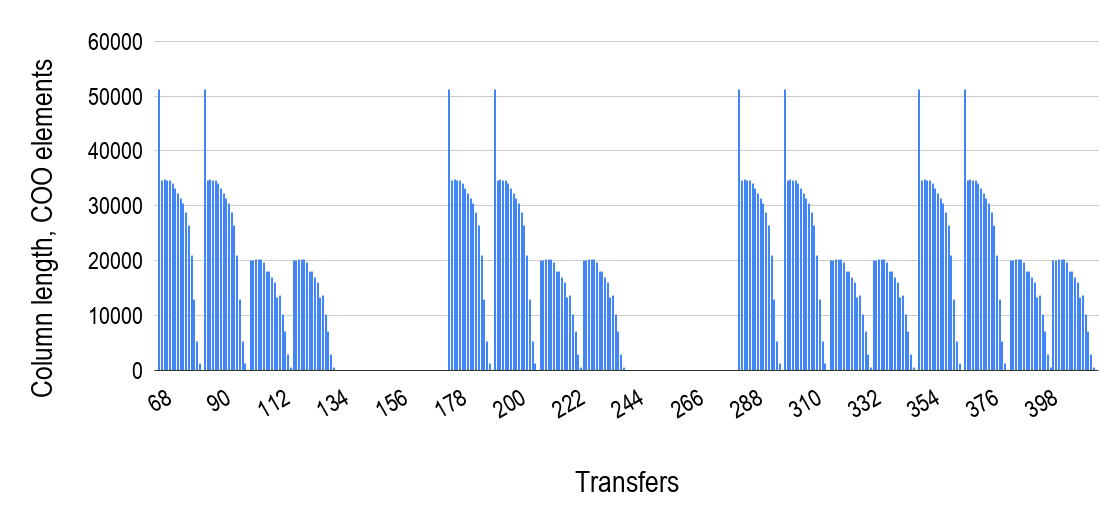
\includegraphics[width=0.7\textwidth]{figures/chapter-3/communication-pattern.png}
        \caption{A part of \textbf{cube-64} communication pattern} \label{fig:communication-pattern}
    \end{figure}

\end{frame}



%%%%%%%%%%%%%%%%%%%%%%%%%%%%%%%%%%%%%%%%%%%%%%%%%%%%%%%%%%
\begin{frame}[t]{Client-Server Process Allocation}
    \small
    \justifying
    
    \begin{itemize}
        \item \text{Three} process allocation \textbf{schemes} were tested on \textbf{HW1 cluster}:
        \begin{itemize}
            \item \textbf{intra-socket} i.e. client and server are distributed within the same socket
            \item \textbf{intra-node} i.e. client and server are distributed among different sockets of the same node
            \item \textbf{inter-node} i.e. client and server are distributed among different nodes
        \end{itemize}
    \end{itemize}

    \begin{figure}[t]
        \centering
        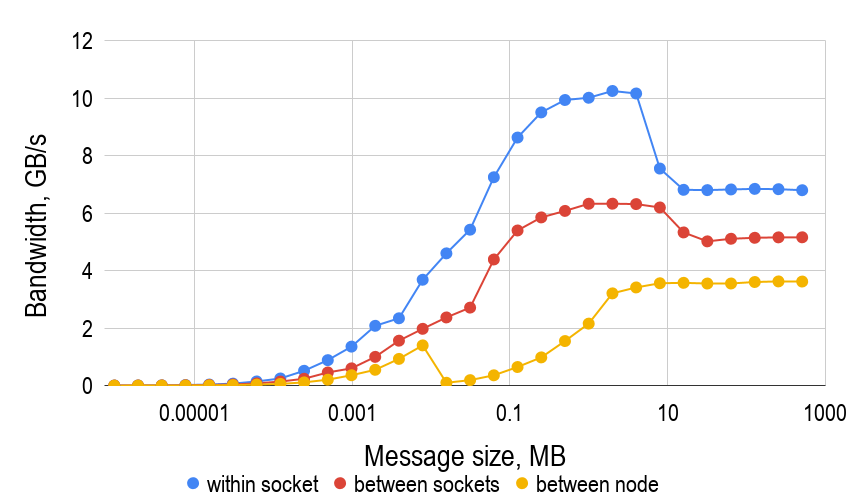
\includegraphics[width=0.55\textwidth]{figures/chapter-3/hw1-bandwidth.png}
    \end{figure}

\end{frame}
\fi
\ifWithResults
\subsection{Results}



%%%%%%%%%%%%%%%%%%%%%%%%%%%%%%%%%%%%%%%%%%%%%%%%%%%%%%%%%%
\begin{frame}[t]{Communication pattern of \textit{cube-64; N = 100657; F = 1}}
    \footnotesize
    
    \begin{figure}[htpb]
        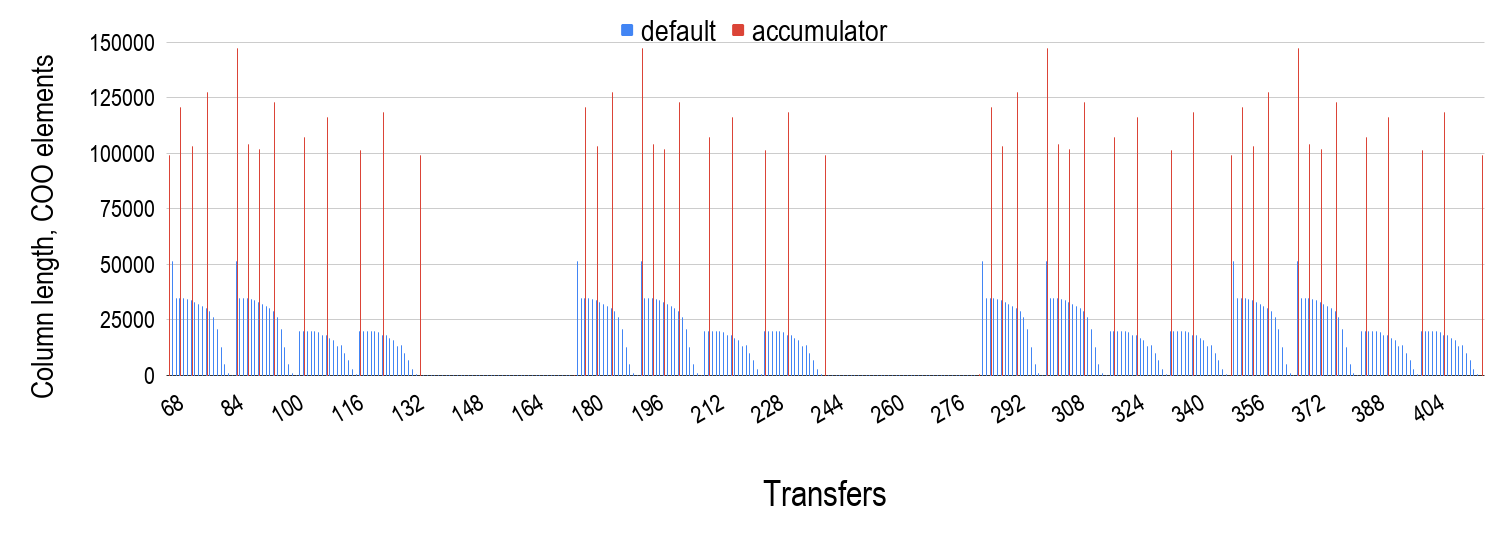
\includegraphics[width=0.9\textwidth]{figures/chapter-3/benchmark-communication-pattern.png}
    \end{figure}
    
    For this particular pattern snippet:
    \begin{itemize}
        \item The amount of data transfers dropped in \textbf{6 times}
        \item From \textbf{344} to \textbf{51}
        \item The average column length increased from \textbf{118114} to \textbf{961186}
        \item or from \textbf{1.8 MB} to \textbf{14.7 MB}
    \end{itemize}

\end{frame}


%%%%%%%%%%%%%%%%%%%%%%%%%%%%%%%%%%%%%%%%%%%%%%%%%%%%%%%%%%
\begin{frame}[t]{Results of Intra-node Allocation}
    \footnotesize
    
    \begin{figure}[htpb]
        \centering
	    \begin{tabular}{c}
		    \subfloat[BM1: blocking MPI; Improved by 9.04\%]{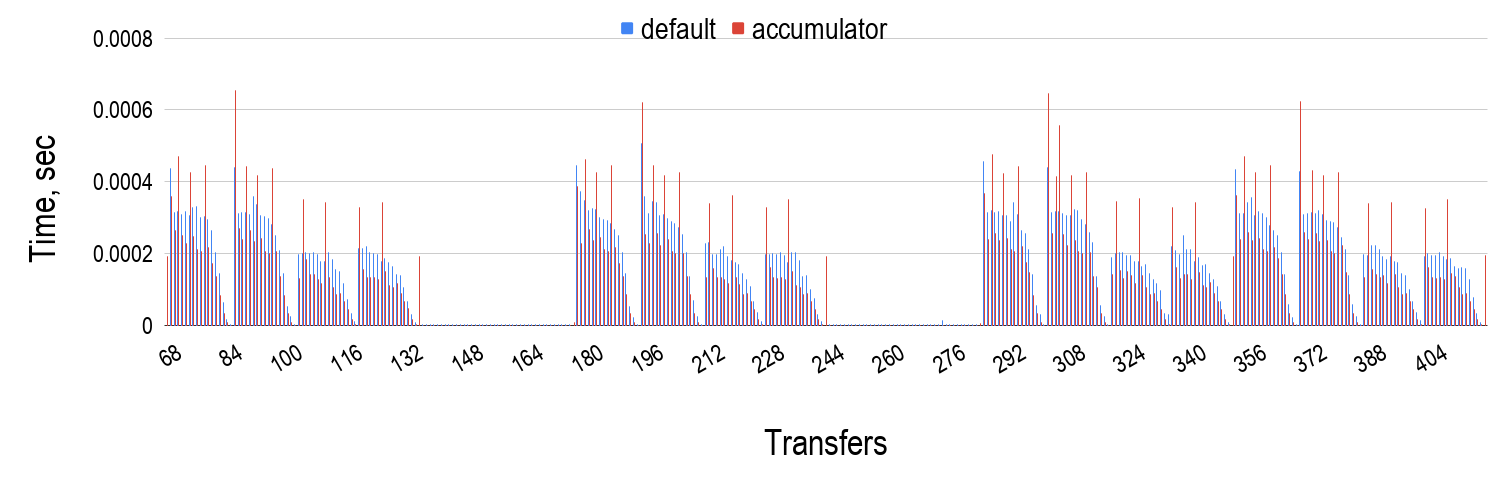
\includegraphics[width=0.7\textwidth]{figures/chapter-3/benchmark-result-blocking.png}} \\
		    \subfloat[BM2: non\-blocking MPI; Improved by  26.26\%]{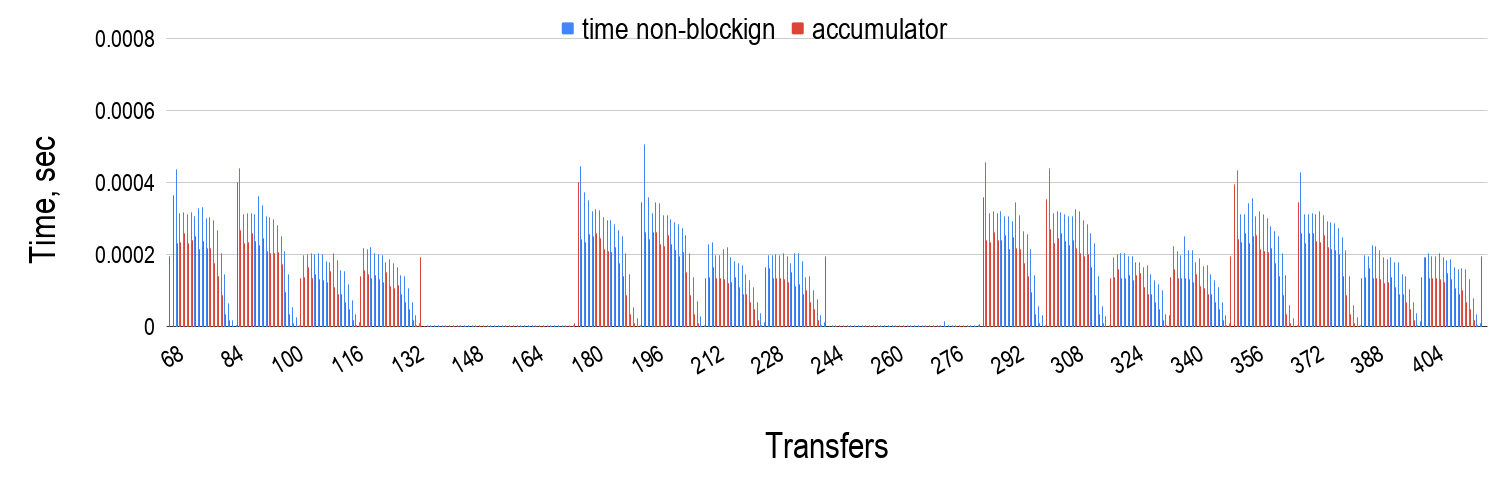
\includegraphics[width=0.7\textwidth]{figures/chapter-3/benchmark-result-non-blocking.png}}
	    \end{tabular}
    	
	\label{fig:benchmark:results-cube-64}
\end{figure}

\end{frame}


%%%%%%%%%%%%%%%%%%%%%%%%%%%%%%%%%%%%%%%%%%%%%%%%%%%%%%%%%%
\begin{frame}[t]{Results of Intra/Inter- Socket/Node Allocation: +}
    \small
    \begin{table}[ht]
    \centering
        \begin{tabular}{|c|c|c|}
        \hline
        \begin{tabular}[c]{@{}c@{}}Benchmark\\ name\end{tabular} & BM1, \% & BM2, \% \\ \hline
    within a socket                                          & 7.61    & 13.84   \\ \hline
    among sockets                                          & 9.04    & 26.26   \\ \hline
    among nodes                                            & -2.06   & 3.20    \\ \hline
    \end{tabular}
    \caption{Time reduction in comparison with the default approach}
        \label{table:benchmark:performance-gain}
    \end{table}
    
    \normalsize
    \begin{itemize}
        \setlength\itemsep{0.5cm}

        \item The new concept \textbf{always} results in some \textbf{performance improvement} 
        \item The \textbf{main} performance \textbf{gain} comes from computation/communication \textbf{overlap}

    \end{itemize}

\end{frame}


%%%%%%%%%%%%%%%%%%%%%%%%%%%%%%%%%%%%%%%%%%%%%%%%%%%%%%%%%%
\begin{frame}[t]{Results of Intra/Inter- Socket/Node Allocation: --}
    \small
    \begin{table}[ht]
    \centering
        \begin{tabular}{|c|c|c|}
        \hline
        \begin{tabular}[c]{@{}c@{}}Benchmark\\ name\end{tabular} & BM1, \% & BM2, \% \\ \hline
    within a socket                                          & 7.61    & 13.84   \\ \hline
    among sockets                                          & 9.04    & 26.26   \\ \hline
    among nodes                                            & -2.06   & 3.20    \\ \hline
    \end{tabular}
    \caption{Time reduction in comparison with the default approach}
    \end{table}
    
    \begin{itemize}
        \item \textbf{Negative effect} of data \textbf{accumulation} in case of \textbf{inter-node} communication
        \item \textbf{Negligible performance gain} out of non-blocking data transfer in case of \textbf{inter-node communication}
        \item \textbf{Specifics} of the benchmark? MPI \textbf{Eager} and \textbf{Rendezvous} protocol switching?
    \end{itemize}

\end{frame}



%%%%%%%%%%%%%%%%%%%%%%%%%%%%%%%%%%%%%%%%%%%%%%%%%%%%%%%%%%
\begin{frame}[t]{Specifics of Benchmarks}
    \small
    \begin{table}[ht]
    \centering
        \begin{tabular}{|c|c|c|}
        \hline
        \begin{tabular}[c]{@{}c@{}}Benchmark\\ name\end{tabular} & BM1, \% & BM2, \% \\ \hline
    within a socket                                          & 7.61    & 13.84   \\ \hline
    among sockets                                          & 9.04    & 26.26   \\ \hline
    among nodes                                            & -2.06   & 3.20    \\ \hline
    \end{tabular}
    \caption{Time reduction in comparison with the default approach}
    \end{table}
    
    \begin{figure}[htpb]
        \centering
        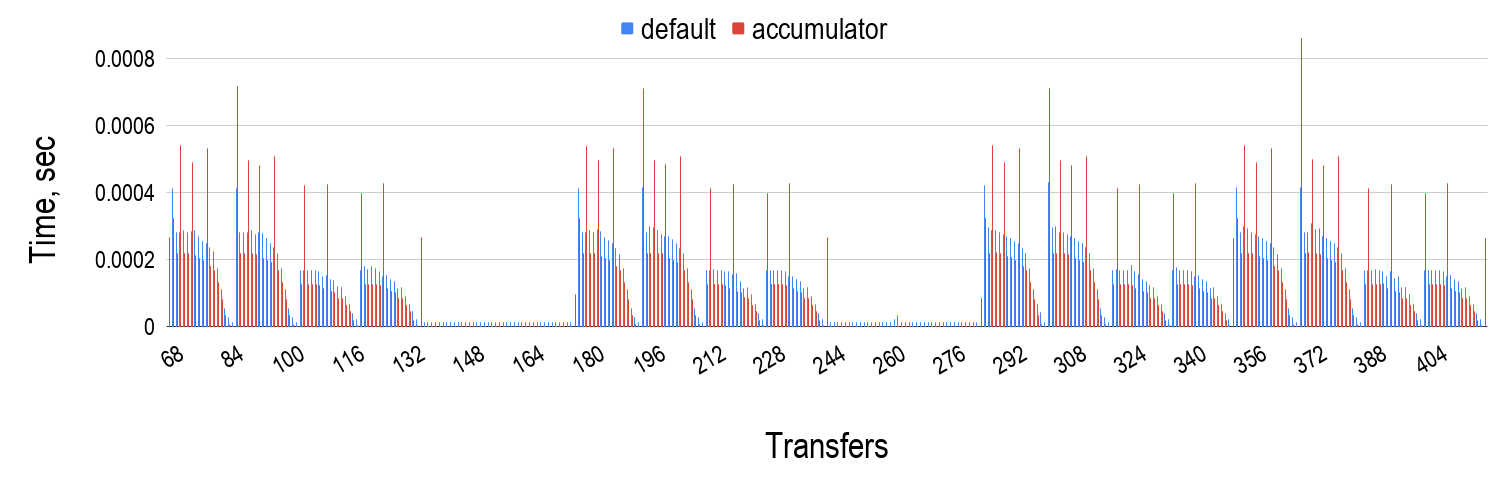
\includegraphics[width=0.8\textwidth]{figures/chapter-3/benchmark-result-non-blocking-inter-node-comm.png}
        \caption{\textbf{Inter-node} communication in case of \textbf{cube-64}}
        \label{fig:benchmark:results-cube-64-inter-node-comm}
\end{figure}
\end{frame}



%%%%%%%%%%%%%%%%%%%%%%%%%%%%%%%%%%%%%%%%%%%%%%%%%%%%%%%%%%
\begin{frame}[t]{Specifics of Benchmarks}
    \small
    \begin{table}[ht]
    \centering
        \begin{tabular}{|c|c|c|}
        \hline
        \begin{tabular}[c]{@{}c@{}}Benchmark\\ name\end{tabular} & BM1, \% & BM2, \% \\ \hline
    within a socket                                          & 7.61    & 13.84   \\ \hline
    among sockets                                          & 9.04    & 26.26   \\ \hline
    among nodes                                            & -2.06   & 3.20    \\ \hline
    \end{tabular}
    \caption{Time reduction in comparison with the default approach}
    \end{table}
    
    \begin{itemize}
        \item Running the benchmarks with \textit{cube-645; N = 100657; F = 1}
        \item size(\textit{cube-645}) $\approx$ 10 $\cdot$  size( \textit{cube-64} )
        \item Performance of BM1 dropped by \textbf{-6.35\%}
        \item Performance of BM2 improved by \textbf{+23.21\%}
    \end{itemize}

\end{frame}

%%%%%%%%%%%%%%%%%%%%%%%%%%%%%%%%%%%%%%%%%%%%%%%%%%%%%%%%%%
\begin{frame}[t]{To consider}
    \justifying
    \small
    \begin{itemize}
        \item Time spent on data transfer is approximately \textbf{one fifth of the total time}
        \item Data transfer happens \textbf{too fast!}
        \item It is just a simple \textbf{benchmark} which \textbf{generates} column vectors filled with \textbf{random numbers}
    \end{itemize}
    
    \begin{figure}[htpb]
        \centering
        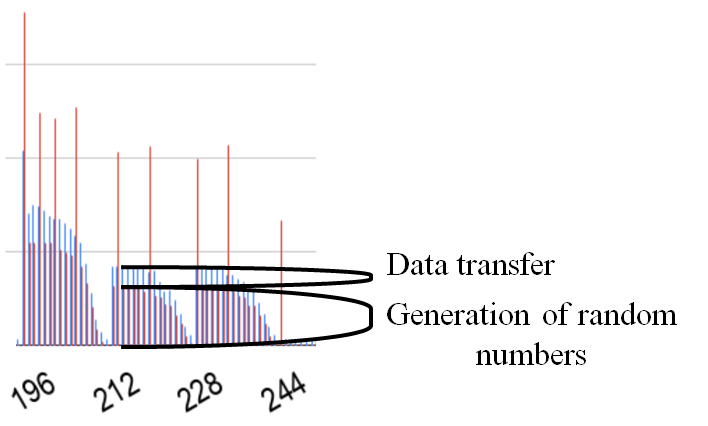
\includegraphics[width=0.6\textwidth]{figures/chapter-3/fast-data-transfer.png}
        \caption{\textbf{Intra-node} communication in case of \textbf{cube-64}}
    \end{figure}

\end{frame}
\fi
%\ifWithResults

\subsection{Results and Conclusion}

%%%%%%%%%%%%%%%%%%%%%%%%%%%%%%%%%%%%%%%%%%%%%%%%%%%%%%%%%%
\begin{frame}[t]{Results: Benchmarks}
 \small
    \begin{table}[ht]
    \centering
        \begin{tabular}{|c|c|c|}
        \hline
        \begin{tabular}[c]{@{}c@{}}Benchmark\\ name\end{tabular} & BM1, \% & BM2, \% \\ \hline
    within a socket                                          & 7.61    & 13.84   \\ \hline
    among sockets                                          & 9.04    & 26.26   \\ \hline
    among nodes                                            & -2.06   & 3.20    \\ \hline
    \end{tabular}
    \caption{Time reduction in comparison with the default approach}
        \label{table:benchmark:performance-gain}
    \end{table}

    \vspace{-20.0pt}
    \begin{figure}[htpb]
        \centering
        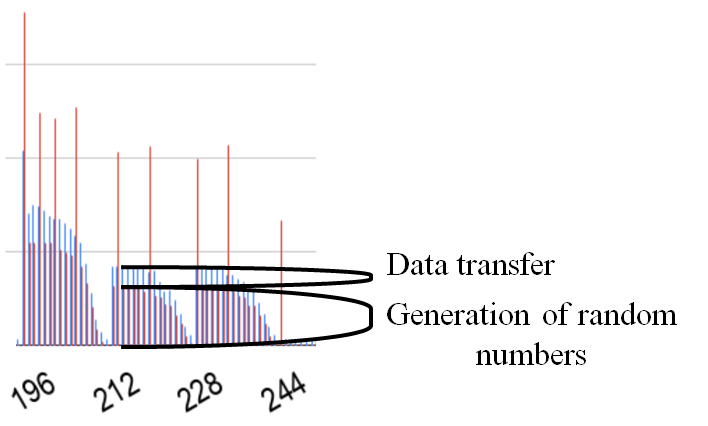
\includegraphics[width=0.6\textwidth]{figures/chapter-3/fast-data-transfer.png}
        \caption{\textbf{Intra-node} communication in case of \textbf{cube-64}}
    \end{figure}
\end{frame}

%%%%%%%%%%%%%%%%%%%%%%%%%%%%%%%%%%%%%%%%%%%%%%%%%%%%%%%%%%
\begin{frame}[t]{Results: ATHLET}
    \small
    \justifying
    
    \begin{itemize}
        \item Ideas, expressed in \textbf{BM2} benchmark,  were \textbf{implemented in ATHLET-NuT}
        
        \item Several simulation scenarios were taken for the final \textbf{verification and performance} testing
        
        \item \textbf{Verification} of the modified code \textbf{did not detect any deviations} of numerical results
        
        \item All tests showed  \textbf{considerable improvement} with respect to the \textit{\textbf{communication time}} i.e. approximately in \textbf{50-60\%}
    \end{itemize}

    \begin{table}[ht]
        \centering
        \begin{tabular}{|c|c|c|c|}
        \hline
Test case                                                    & \multicolumn{3}{c|}{pwr-3d}           \\ \hline
Type & intra-soket & intra-node & inter-node \\ \hline
Time reduction, \%                                           & 42.55\%     & 66.17\%    & 76.03\%    \\ \hline
        \end{tabular}
        \caption{ATHLET Results of \textbf{pwr-3d} test case}
    \end{table}

\end{frame}


%%%%%%%%%%%%%%%%%%%%%%%%%%%%%%%%%%%%%%%%%%%%%%%%%%%%%%%%%%
\begin{frame}[t]{Results: Overall Performance improvement}
    \spc
    \justifying
    
        \begin{itemize}
            \setlength\itemsep{0.25cm}
            \item \textbf{Overall improvement} of applied changes \textbf{achieved} only \textbf{0.14\% in average}, regardless of client-server allocation
            
            \item \textbf{Profiling} showed the \textbf{communication} part of the original implementation \textbf{took} around \textbf{0.24\%} of the \textbf{total} matrix evaluation-transfer \textbf{time}
            
            \item \textbf{Computation} part takes almost \textbf{99.8\%}
        \end{itemize}
    
    \begin{block}{According to BM2 benchmark:}
        \begin{itemize}
            \item Time spent on data transfer is approximately \textbf{one fifth of the total time}
            
            \item The benchmark \textbf{generates} only \textbf{random numbers}
        \end{itemize}
    \end{block}
    
\end{frame}


%%%%%%%%%%%%%%%%%%%%%%%%%%%%%%%%%%%%%%%%%%%%%%%%%%%%%%%%%%
\begin{frame}[t]{Conclusion}
    \small
    \justifying
    
    \begin{itemize}
            \item The \textbf{initial goal} of improvement ATHLET-NuT communication during the compressed Jacobian transfers \textbf{has been achieved}
            \item \textbf{Negligible} overall performance \textbf{gain}
            \begin{itemize}
                \item A \textbf{wrong Hypotheses} at the beginning
                \item Absence of \textbf{Initial Profiling}
            \end{itemize}
    \end{itemize}
    
        \begin{figure}[htpb]
        \centering
        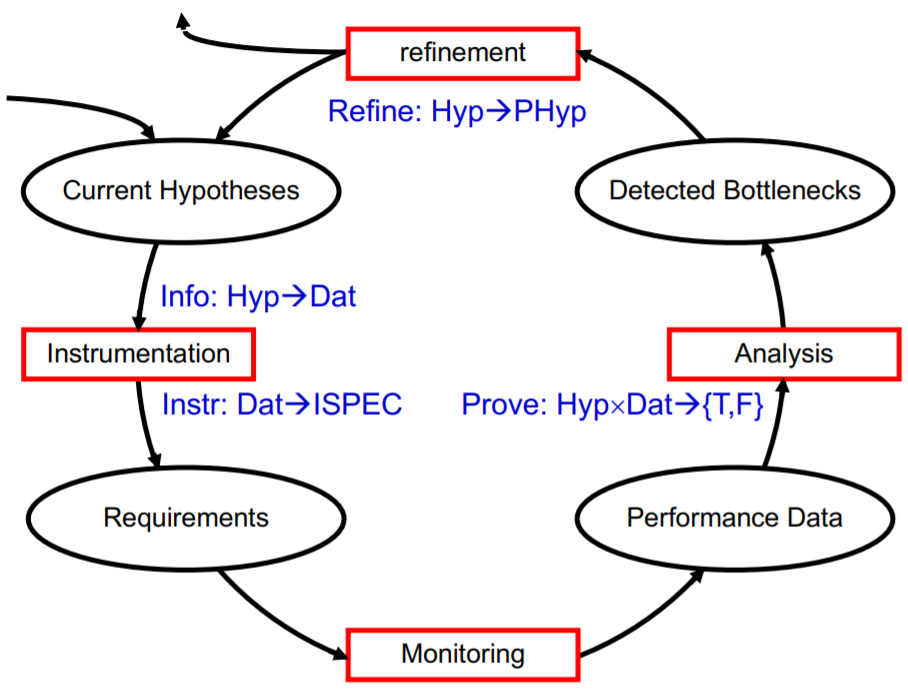
\includegraphics[width=0.44\textwidth]{figures/chapter-3/Performance-analysis.png}
        \caption{performance analysis framework \cite{perfomance-analysis-framework}}
    \end{figure}

\end{frame}
%\fi


%%%%%%%%%%%%%%%%%%%% THANKY %%%%%%%%%%%%%%%%%%%%
\begin{frame}{}
    \centering
    \Large
  \emph{Thanks for your attention!}
\end{frame}


\begin{frame}[allowframebreaks]
        \printbibliography{}
\end{frame}


\end{document}